\documentclass[11pt]{article}

\usepackage[T1]{fontenc}
\usepackage{amsmath}
\usepackage{amssymb}
\usepackage{amsthm}
\usepackage{booktabs}
\usepackage{microtype}
\usepackage[margin=1in]{geometry}
\usepackage{xcolor}
\usepackage{tikz}
\usetikzlibrary{arrows.meta,calc,positioning,decorations.pathreplacing,fit,backgrounds,shapes.misc}
\usepackage{tikz-cd}
\usepackage[hidelinks]{hyperref}

\newtheorem{theorem}{Theorem}[section]
\newtheorem{lemma}[theorem]{Lemma}
\newtheorem{proposition}[theorem]{Proposition}
\newtheorem{corollary}[theorem]{Corollary}
\newtheorem{definition}[theorem]{Definition}
\newtheorem{remark}[theorem]{Remark}
\newtheorem{example}[theorem]{Example}
\newtheorem{mainthm}{Theorem}
\renewcommand{\themainthm}{\Alph{mainthm}}

\newcommand{\R}{\mathbb R}
\newcommand{\Opt}{\operatorname{Opt}}
\newcommand{\cl}{\operatorname{cl}}
\newcommand{\blk}{\operatorname{blk}}
\newcommand{\PO}{\mathrm{PO}}
\newcommand{\Bases}{\mathcal B}
\newcommand{\Pos}{\mathcal P}
\newcommand{\CC}{\mathcal C}
\newcommand{\Av}{\operatorname{Av}}
\newcommand{\STrop}{\operatorname{size}_{\max,+,-}}
\newcommand{\Bool}{\operatorname{size}_{\mathrm{Bool}}}

\definecolor{acc}{RGB}{28,92,160}
\definecolor{accl}{RGB}{226,236,248}
\definecolor{wrm}{RGB}{186,74,26}
\definecolor{grl}{RGB}{238,238,238}

\tikzset{
  >={Stealth[length=2.1mm,width=1.5mm]},
  every picture/.style={line cap=round,line join=round},
  dotS/.style={circle,draw=black,fill=black,inner sep=0pt,minimum size=5.2pt},
  dotO/.style={circle,draw=black,fill=white,inner sep=0pt,minimum size=5.2pt,line width=0.6pt},
  dotX/.style={cross out,draw=black!55,inner sep=0pt,minimum size=4.4pt,line width=0.8pt},
  axis/.style={->,line width=0.6pt,black!80},
  lab/.style={font=\footnotesize},
  slab/.style={font=\scriptsize},
}

\title{Greedy and Matroid Intersection\\without Branching}
\author{Shuhuan Wang\\{\small\texttt{ukiyo7@gmail.com}}}
\date{}

\begin{document}
\maketitle

\begin{abstract}
The greedy algorithm and the augmenting path algorithms of matroid optimization
compare weights and branch on the outcome.  A $(\max,+,-)$-circuit, like a ReLU
network, computes a continuous function and cannot branch; we show that both
algorithms have exact counterparts of polynomial size.  For a matroid on $m$
elements, a Boolean circuit of size $s$ for the rank function yields a
$(\max,+,-)$-circuit of size $3ms+O(m^{2})$ for the maximum weight of a base, and
the two complexities are polynomially equivalent.  Both are polynomial for binary
matroids, matroids represented over $\mathbb Q$ or a fixed finite field, and
gammoids.  For two matroids with rank circuits of sizes $s_1$ and $s_2$, circuits
of size $O(m^{7}(s_1+s_2+m))$ compute the optimal values of weighted matroid
intersection, including the assignment problem, for which polynomial size was
open.  The circuit updates Lagrange multipliers in a fixed sequence.  The family
of bases these updates should test is NP-hard to query in general, but a
monotone family of matroids containing it keeps the updates valid; a potential
bounds their number.  All circuits and size bounds are verified in Lean~4.
\end{abstract}

\section{Introduction}
\label{sec:intro}

The greedy algorithm for weighted bases~\cite{edmonds71} and the augmenting path
algorithms for weighted matroid
intersection~\cite{edmonds70,lawler75,frank81} decide what to do next by
comparing weights.  A circuit over $\max$, $+$ and $-$ cannot do that: it
computes a continuous function of its inputs, and the answer to a comparison is
discontinuous.  Circuits over $\min$ and $+$ alone, which model pure dynamic
programming, pay exponentially for the missing comparisons.  Jukna and
Seiwert~\cite{jukna-seiwert18-greedy} prove that minimum spanning tree, solved by
the greedy algorithm, needs $(\min,+)$-circuits of size $2^{\Omega(\sqrt n)}$ on
$n$-vertex graphs, and minimum-cost arborescence and the assignment problem need
size $2^{\Omega(n)}$ by Jerrum and Snir~\cite{jerrum-snir82}.  Jukna surveys the
model~\cite{jukna15-tropical,jukna23-tropical}.

With subtraction, Hertrich and Sering~\cite{hertrich-sering25} obtain
polynomial-size circuits for
the minimum spanning tree value and for maximum flow.  Fomin, Grigoriev and
Koshevoy~\cite{fgk16} construct small subtraction-free circuits for the
generating polynomials of spanning trees and of directed spanning trees;
tropicalizing them gives polynomial-size $(\min,+,-)$-circuits for minimum-cost
arborescence.  Hertrich, Kober and
Loho~\cite{hertrich-kober-loho26} tropicalize a small circuit for the basis
generating polynomial of a regular matroid and name binary matroids as the
natural next step, noting that counting their bases is \#P-hard and that
different techniques would be needed.  By the identity
$\max(a,b)=\max(0,a-b)+\max(0,b)-\max(0,-b)$, a $(\max,+,-)$-circuit of size $S$
converts into a ReLU neural network of size $3S$~\cite{hertrich-kober-loho26},
so every circuit below also yields an exact ReLU neural network.

Our circuits read matroids through their rank functions rather than their
generating polynomials.  Weighted bases of any matroid and weighted
intersection of any two matroids get exact circuits of polynomial size whenever
the rank functions have Boolean circuits of polynomial size.
Figure~\ref{fig:map} shows where the results sit.

\begin{figure}[t]
  \centering
  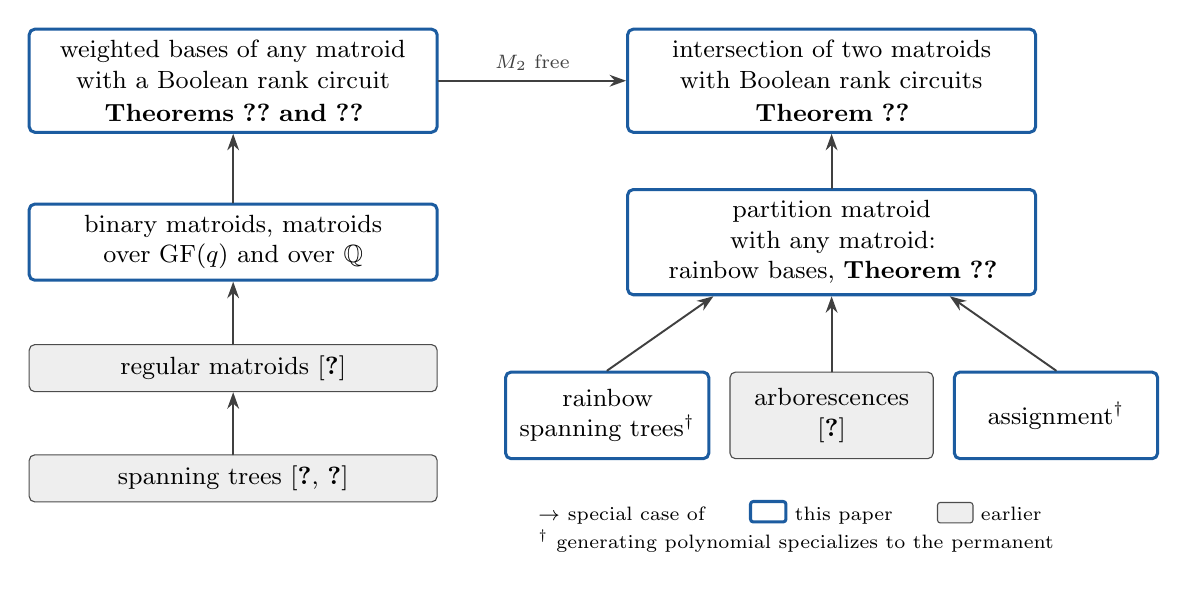
\begin{tikzpicture}[
      box/.style={draw=black!70,rounded corners=2pt,align=center,font=\small,
        inner sep=4pt,text width=#1},
      box/.default=49mm,
      old/.style={box=#1,fill=grl},
      old/.default=49mm,
      new/.style={box=#1,draw=acc,line width=1.1pt,fill=white},
      new/.default=49mm,
      sp/.style={->,line width=0.7pt,black!75},
      tag/.style={font=\scriptsize,fill=white,inner sep=1.2pt}]
    \node[new] (A) at (0,0)
      {weighted bases of any matroid\\with a Boolean rank circuit\\[1pt]
       \textbf{Theorems~\ref{thm:A} and \ref{thm:B}}};
    \node[new] (bin) at (0,-2.05) {binary matroids, matroids\\over $\mathrm{GF}(q)$ and over $\mathbb Q$};
    \node[old] (reg) at (0,-3.65) {regular matroids~\cite{hertrich-kober-loho26}};
    \node[old] (mst) at (0,-5.05) {spanning trees~\cite{hertrich-sering25,fgk16}};
    \node[new] (D) at (7.6,0)
      {intersection of two matroids\\with Boolean rank circuits\\[1pt]
       \textbf{Theorem~\ref{thm:D}}};
    \node[new] (C) at (7.6,-2.05)
      {partition matroid with any matroid:\\rainbow bases, \textbf{Theorem~\ref{thm:C}}};
    \node[new=23mm,minimum height=11mm] (rst) at (4.75,-4.25)
      {rainbow\\spanning trees$^{\dagger}$};
    \node[old=23mm,minimum height=11mm] (arb) at (7.6,-4.25)
      {arborescences\\\cite{fgk16}};
    \node[new=23mm,minimum height=11mm] (asg) at (10.45,-4.25)
      {assignment$^{\dagger}$};
    \draw[sp] (bin) -- (A);
    \draw[sp] (reg) -- (bin);
    \draw[sp] (mst) -- (reg);
    \draw[sp] (C) -- (D);
    \draw[sp] (rst.north) -- ([xshift=-15mm]C.south);
    \draw[sp] (arb.north) -- (C.south);
    \draw[sp] (asg.north) -- ([xshift=15mm]C.south);
    \draw[sp] (A.east) -- node[tag,above=2pt] {$M_2$ free} (D.west);
    \node[font=\scriptsize,align=left,anchor=north west] at (3.75,-5.2)
      {$\to$\ special case of\qquad
       \raisebox{-0.35ex}{\tikz\draw[draw=acc,line width=1.1pt,rounded corners=1pt]
         (0,0) rectangle (4.5mm,2.6mm);}\ this paper\qquad
       \raisebox{-0.35ex}{\tikz\draw[draw=black!70,fill=grl,rounded corners=1pt]
         (0,0) rectangle (4.5mm,2.6mm);}\ earlier\\[2pt]
       $^{\dagger}$\ generating polynomial specializes to the permanent};
  \end{tikzpicture}
  \caption{Problems over $\max,+,-,0$ treated here and before.  Arrows point
  from a special case to a more general problem.  Gray boxes were obtained by
  tropicalizing small subtraction-free circuits~\cite{fgk16,hertrich-kober-loho26}
  or by direct constructions~\cite{hertrich-sering25}.  The
  problems marked $\dagger$ contain the permanent and binary matroids have a
  \#P-hard basis count; for none of them is a small subtraction-free circuit of
  the generating polynomial known.}
  \label{fig:map}
\end{figure}

\paragraph{Greedy without branching.}
Let $M$ be a matroid on a ground set $E$ with $|E|=m$, rank function $r$,
rank $k=r(E)$ and set of bases $\Bases(M)$.  For $u\in\R^{E}$ and $X\subseteq E$
write $u(X)=\sum_{e\in X}u_e$, and let
\[
  h_M(w)=\max_{B\in\Bases(M)}w(B)
\]
be the largest weight of a base.  Put $L=\lceil\log_2(k+1)\rceil$, the number
of binary digits of $k$.  Our circuits read $M$ only through a \emph{Boolean rank
circuit}, a Boolean circuit that outputs the binary digits of $r(X)$ from the
indicator vector of $X\subseteq E$.

\begin{mainthm}[Maximum-weight bases]
\label{thm:A}
If $M$ has a Boolean rank circuit of size $s$, then a $(\max,+,-)$-circuit of
size at most
\[
  3ms+mL+9m^{2}+4m+4L+1
\]
computes $h_M(w)$ at every $w\in\R^{E}$.
\end{mainthm}

\begin{mainthm}[Converse]
\label{thm:B}
If a $(\max,+,-)$-circuit of size $S$ computes $h_M$ on $\{0,1\}^{E}$, then $M$
has a Boolean rank circuit of size at most $15S^{2}+40S$.
\end{mainthm}

So, for every matroid, the $(\max,+,-)$-circuit complexity of $h_M$ and the
Boolean circuit complexity of its rank function are polynomially related, in
both directions (Corollary~\ref{cor:equiv}).  A binary matroid represented by an
$n\times m$ matrix has a Boolean rank circuit of size $O(mn^{2})$ by Gaussian
elimination without branching.  The same elimination over a field with $q$
elements costs $O(q^{2}mn^{2})$ gates, graphic matroids are binary, matroids
represented over $\mathbb Q$ by integer matrices with entries of $b$ bits have
rank circuits of size polynomial in $m$, $n$ and $b$, and passing to the dual
costs $O(m\log m)$ gates (Corollary~\ref{cor:classes}).  Transversal matroids
and gammoids have rank circuits of polynomial size through the matroid
intersection circuit of Section~\ref{sec:circuit}
(Corollary~\ref{cor:transversal}).
By counting, most matroids need $(\max,+,-)$-circuits of size $2^{m/2-O(\log m)}$
(Corollary~\ref{cor:count}).

\paragraph{Matroid intersection without branching.}
Let the ground set of $M$ be partitioned into blocks $R_1,\ldots,R_k$, where $k$
is the rank of $M$.  A set is \emph{rainbow} if it meets every block at most
once, so a rainbow base meets every block once, and we write
\[
  \Opt(w)=\min\{\,w(B):B\text{ a rainbow base of }M\,\}.
\]
Rainbow spanning trees are the rainbow bases of a graphic matroid with colored
edges.  Arborescences are the rainbow bases of a graphic matroid whose blocks are
the in-arcs of the non-root vertices.

\begin{mainthm}[Rainbow bases]
\label{thm:C}
If $M$ has a Boolean rank circuit of size $s$ and a rainbow base, then a uniform
$(\max,+,-)$-circuit of size $O(k^{3}m^{4}(s+m))$ computes $\Opt(w)$ at every
$w\in\R^{E}$.
\end{mainthm}

\begin{mainthm}[Weighted matroid intersection]
\label{thm:D}
Let $M_1$ and $M_2$ be matroids on $E$, $|E|=m$, with Boolean rank circuits of
sizes $s_1$ and $s_2$.  If they have a common base, a uniform $(\max,+,-)$-circuit of size $O(m^{7}(s_1+s_2+m))$ computes the minimum weight of a common base
at every $w\in\R^{E}$.  For all such $M_1$ and $M_2$, one of size $O(m^{7}(s_1+s_2+m))$ computes
the maximum weight of a common independent set.
\end{mainthm}

Theorem~\ref{thm:D} follows from Theorem~\ref{thm:C} through the classical
correspondence between common bases of $M_1,M_2$ and rainbow bases of
$M_1\oplus M_2^{*}$ on two copies of $E$, and common independent sets become
common bases once $m$ free elements are added (Section~\ref{sec:two}).

For the $n\times n$ assignment problem, the ground set consists of the $n^{2}$
entries of the cost matrix, $M$ is the partition matroid with one part per
column, which has a Boolean rank circuit of size $O(n^{2})$ (one disjunction per
column and a population count), and the blocks are the rows.  Every connected
component of $M$ is a column of rank one, so Corollary~\ref{cor:rankone} and the
proof of Theorem~\ref{thm:C} give $(\max,+,-)$-circuits, and hence ReLU neural
networks, of size $O(k^{3}m^{3}(s+m))=O(n^{11})$.  Hertrich and
Sering~\cite{hertrich-sering25} and
Jukna~\cite[Section~6.5, Problem~3]{jukna23-tropical} ask whether polynomial
size is possible for this problem, and Hertrich and
Stargalla~\cite{hertrich-stargalla26}, who list it as open, prove that circuits
over $\max$, $+$ and multiplication by positive scalars need $2^{\Omega(n)}$
addition gates for it.

\paragraph{The update.}
The circuit maintains block potentials $p\in\R^{k}$ and, with $\blk(e)$ the block
of $e$, the Lagrangian
\[
  \Psi(p)=\sum_{b}p_b+\min_{B\in\Bases(M)}\sum_{e\in B}\bigl(w_e-p_{\blk(e)}\bigr),
\]
which is at most $\Opt(w)$ and equals it once some minimum base of the shifted
weights $v_e=w_e-p_{\blk(e)}$ is rainbow.  For $r=1,\ldots,k-1$,
stage $r$ raises the potentials until some minimum base of $v$ meets $r+1$
blocks.  One update raises the potential of each block $b$ by the length of the
set of levels $t\ge0$ at which a matroid $N(t)$, read from the pairs $(e,f)$ with
$v_f-v_e\le t$, has a base that meets exactly $r$ blocks and misses
$b$, counted up to the first level at which $N(t)$ has a base meeting $r+1$
blocks.  Such a length is an integral over $t$ of Boolean tests, and
Corollary~\ref{cor:levels} turns a Boolean circuit for the tests into a
$(\max,+,-)$-circuit for the integral.

\paragraph{Which family.}
The exact family for these tests is the family $\Pos_t$ of bases that are optimal for
some weight within $t/2$ of $v$ in every coordinate, the possibly optimal bases
of interval data~\cite{kasperski08}.  It is not a matroid, and
deciding whether it contains a rainbow spanning tree is NP-complete
(Proposition~\ref{prop:nphard}), so we enlarge it.
Theorem~\ref{thm:validity} shows that for every monotone family of matroids that
starts at the minimum bases and contains $\Pos_t$, each update raises $\Psi$ by
exactly $k-r$ times its length, and every minimum base that meets $r$ blocks
stays minimum.  The family enters only through an upper bound on how many
raised elements a minimum base can hold, and matroid intersection supplies that
bound.  The family we use clusters the possibly optimal elements of each
connected component by single linkage at scale $t$
(Proposition~\ref{prop:posl}).  Each $N(t)$ of this family is a matroid read from the pairs $(e,f)$ with
$v_f-v_e\le t$ alone.  With the larger
family, a stage can take more than one update.
Theorem~\ref{thm:potential} shows that each update still brings some element of
a fully raised block to or below an element of another block that was above it,
while the set of fully raised blocks never shrinks within a stage, and this
bounds a stage by $r(\lfloor m^{2}/4\rfloor+1)$ updates.  One element of the pair
can be taken in a minimum base fixed for the whole stage, and a pair that has
crossed does not cross back, which bounds a stage by
$\min\bigl(1+(r-1)km,\,1+k(2m-k-1)\bigr)$ updates (Theorem~\ref{thm:stagelength});
no bound in terms of $r$ and $k$ alone holds (Proposition~\ref{prop:ladder}).

\paragraph{Breakpoints.}
For fixed weights, this family changes only at the levels where an element becomes
possibly optimal and where two clusters merge, at most $2m$ levels besides $0$.
An element enters at a level computed from the weights by
Theorem~\ref{thm:compiler}, and two clusters merge at a minimax distance built from the entry levels and the weight differences
(Lemma~\ref{lem:events}).  The circuit computes these levels and applies
Corollary~\ref{cor:levels} at them instead of at the $m^{2}$ pairwise differences, which saves a factor $m$
in Theorems~\ref{thm:C} and~\ref{thm:D}.

\paragraph{Related work.}
Besides the works above, Hertrich and Loho~\cite{hertrich-loho26} show that the
virtual extension complexity of a polytope is at most the size of any neural
network that optimizes over it, so Theorem~\ref{thm:A} with Corollary~\ref{cor:classes}(1) and
Theorem~\ref{thm:D} bound it by a polynomial for the base polytope of a binary
matroid and for the common base and common independent set polytopes of two
binary matroids.  The circuits of Fomin, Grigoriev and
Koshevoy~\cite{fgk16} and of Hertrich, Kober and
Loho~\cite{hertrich-kober-loho26} tropicalize generating polynomials.  Ours are
built from Boolean rank circuits, which reaches binary matroids and matroids
represented over finite fields or over $\mathbb Q$ for bases, and weighted
matroid intersection, with the assignment problem, arborescences and rainbow
spanning trees as special cases.  The maximum flow circuits of~\cite{hertrich-sering25} also run a fixed number
of steps, each of which acts only when a guessed residual distance is correct,
and pass bottleneck capacities through $(\max,\min)$ recursions; in our circuits
the length of each step is an integral of Boolean tests, which
Corollary~\ref{cor:levels} computes.  On the algorithmic side,
Edmonds~\cite{edmonds70,edmonds71}, Lawler~\cite{lawler75} and
Frank~\cite{frank81} solve the same problems by comparisons and augmenting paths,
and Kasperski~\cite{kasperski08} studies possibly optimal solutions under
interval data.

\section{Model and tools}
\label{sec:model}

\subsection{Circuits}

\begin{definition}
\label{def:circuits}
A \emph{$(\max,+,-)$-circuit} on inputs $x\in\R^{n}$ is a directed acyclic
graph whose sources are the coordinates of $x$ and the constant $0$, and whose
other nodes are gates $\max(a,b)$, $a+b$ and $a-b$.  A \emph{Boolean circuit}
on $x\in\{0,1\}^{n}$ has the coordinates of $x$ and the constant $0$ as sources
and gates $\wedge$, $\vee$ and $\neg$.  In both, the size is the number of gates;
sources cost nothing.  A Boolean circuit \emph{outputs the
binary digits} of an integer if its output bits, least significant first, are
these digits.  A family of circuits is \emph{uniform} if a
polynomial-time algorithm produces each member from its combinatorial data,
here the ground set, the blocks and the given Boolean rank circuits.
\end{definition}

A $(\max,+,-)$-circuit computes a continuous piecewise linear function with
integer slopes.  The minimum $\min(a,b)=a-\max(a-b,0)$ costs three gates and
$\max(a,0)$ costs one.

\subsection{Matroids}

We use standard matroid terminology~\cite{oxley11,schrijver03}, and write
$\cl$ for the closure operator of $M$, $X+e=X\cup\{e\}$, $X-e=X\setminus\{e\}$, $[k]=\{1,\ldots,k\}$, $\mathbf 1_X$ for the indicator vector of
a set $X$, $\mathbf 1=\mathbf 1_E$ and $\mathbf 1[P]\in\{0,1\}$ for the truth value of a
statement $P$.  For a
base $B$ and $e\notin B$, the \emph{fundamental circuit} $C(B,e)$ is the unique
circuit in $B+e$.  For a weight $u\in\R^{E}$ write
$\beta_M(u)=\min_{B}u(B)$.  The following facts are classical.

\begin{lemma}
\label{lem:minbases}
Let $u\in\R^{E}$.
\begin{enumerate}
  \item A base $B$ is minimum for $u$ if and only if $u_f\le u_e$ whenever
        $e\notin B$ and $f\in C(B,e)$.
  \item A base $B$ is minimum for $u$ if and only if $B\cap\{u\le c\}$ spans
        $\{u\le c\}$ for every $c\in\R$.
  \item The minimum bases of $u$ are the bases of a matroid $M^{u}$.  For a
        minimum base $B$, $e\notin B$ and $f\in B$, the set $B-f+e$ is a minimum
        base if and only if $f\in C(B,e)$ and $u_f=u_e$, so the circuit of $e$ in
        $B+e$ in $M^{u}$ is $\{e\}\cup\{f\in C(B,e):u_f=u_e\}$.
  \item The relation ``$e=f$, or $e$ and $f$ lie on a common circuit'' is an
        equivalence relation, whose classes are the \emph{connected components};
        a loop or a coloop is a component by itself.  Closure, rank and minimum
        bases decompose over components: $e\in\cl(X)$ if and only if
        $e\in\cl(X\cap K)$ for the component $K$ of $e$, $r(X)=\sum_Kr(X\cap K)$,
        and a base $B$ is minimum if and only if every $B\cap K$ is a minimum base
        of $M|K$.  In particular the minimum bases of $u$, and $M^{u}$, depend
        only on the comparisons of $u$ within components.
\end{enumerate}
\end{lemma}

Explicitly, $M^{u}$ is the direct sum, over the values $\ell$ of $u$, of the
matroids $(M|\{u\le\ell\})/\{u<\ell\}$ on the level sets $\{u=\ell\}$, so its
rank function is read from that of $M$: if $\ell_1<\cdots<\ell_q$ are the values
of $u$ and $U_i=\{u\le\ell_i\}$, $U_0=\varnothing$, then
\begin{equation}
  r_{M^{u}}(A)=\sum_{i=1}^{q}\Bigl(r\bigl(U_{i-1}\cup(A\cap\{u=\ell_i\})\bigr)-r(U_{i-1})\Bigr).
  \label{eq:rank-mu}
\end{equation}

\subsection{From Boolean circuits to \texorpdfstring{$(\max,+,-)$}{(max,+,-)}-circuits}

Theorem~\ref{thm:compiler} below turns Boolean circuits into
$(\max,+,-)$-circuits for the sums of Definition~\ref{def:ti}, with explicit
constants.

\begin{definition}
\label{def:ti}
For $D\in\R^{E}_{\ge0}$ and $t\ge0$ let $G_t(D)=\{e:D_e\le t\}$, and let
$0=d_0\le d_1\le\cdots\le d_m$ be the entries of $D$ in increasing order with a
zero prepended.  Let $\Delta_i=d_{i+1}-d_i$.  For
$F:2^{E}\to\R$ let
\[
  \CC_F(D)=\sum_{i=0}^{m-1}\Delta_i\,F\bigl(G_{d_i}(D)\bigr)
  =\int_0^{d_m}F\bigl(G_t(D)\bigr)\,dt.
\]
\end{definition}

The two expressions agree because $G_t(D)=G_{d_i}(D)$ for every $t$ in
$[d_i,d_{i+1})$.  If $F(E)=0$, the upper limit $d_m=\max_eD_e$ can be replaced
by $\infty$, since $G_t(D)=E$ for $t\ge d_m$, and $\CC_F(D)$ is the Lov\'asz
extension of $X\mapsto F(E\setminus X)$ at $D$~\cite{lovasz83}.

\begin{theorem}
\label{thm:compiler}
Let one Boolean circuit of size $s$ compute $F=(F_1,\ldots,F_N):2^{E}\to\{0,1\}^{N}$
from the indicator vector of its argument.  Then a $(\max,+,-)$-circuit of
size at most $3ms+mN+6m^{2}$ computes $(\CC_{F_1}(D),\ldots,\CC_{F_N}(D))$ at
every $D\in\R^{E}_{\ge0}$.
\end{theorem}

\begin{proof}
\emph{Step 1: $d_i$ and $\Delta_i$.}  The insertion sorting network~\cite{knuth98-taocp3} has
$m(m-1)/2$ comparators, each computing
\[
  \max(a,b)\quad\text{and}\quad\min(a,b)=a+b-\max(a,b)
\]
with three gates.  It outputs $d_1,\ldots,d_m$, and one gate per $i<m$ gives
$\Delta_i=d_{i+1}-d_i$.

\emph{Step 2: $\Delta_i\mathbf 1[e\in G_{d_i}(D)]$.}  For $i<m$ and $e\in E$, the entry $D_e$
occurs in the sorted list, so $D_e\le d_i$ or $D_e\ge d_{i+1}$, and
\begin{equation}
  \max\bigl(\Delta_i-\max(D_e-d_i,0),\,0\bigr)
  =\begin{cases}\Delta_i,&D_e\le d_i\\0,&D_e\ge d_{i+1}\end{cases}
  =\Delta_i\,\mathbf 1\bigl[e\in G_{d_i}(D)\bigr],
  \label{eq:bit}
\end{equation}
at four gates.

\emph{Step 3: $\Delta_iF_j(G_{d_i}(D))$.}  For $\Delta=\Delta_i\ge0$ and $x,y\in\{0,1\}$,
\[
  \max(\Delta x+\Delta y-\Delta,0)=\Delta(x\wedge y),\quad
  \max(\Delta x,\Delta y)=\Delta(x\vee y),\quad
  \Delta-\Delta x=\Delta(\neg x).
\]
Let $B$ be the given Boolean circuit and $B_\Delta$ the circuit in which each gate of
$B$ is replaced by the left side, at most three gates.  By induction on the gates,
\[
  \begin{tikzcd}[column sep=4.5em,row sep=2.2em]
    \{0,1\}^{E}\arrow[r,"B"]\arrow[d,"\Delta\,\cdot"'] & \{0,1\}^{N}\arrow[d,"\Delta\,\cdot"]\\
    \R^{E}\arrow[r,"B_\Delta"'] & \R^{N}
  \end{tikzcd}
\]
commutes, and at the inputs of \eqref{eq:bit}
\[
  B_\Delta\bigl(\Delta\mathbf 1_{G_{d_i}(D)}\bigr)=\Delta B\bigl(\mathbf 1_{G_{d_i}(D)}\bigr)
  =\Delta_iF\bigl(G_{d_i}(D)\bigr).
\]

\emph{Step 4: $\CC_{F_j}(D)$ with at most $3ms+mN+6m^{2}$ gates.}  With $N$ additions for each $i$,
\[
  \sum_{i=0}^{m-1}\Delta_iF_j\bigl(G_{d_i}(D)\bigr)=\CC_{F_j}(D),\qquad j=1,\ldots,N,
\]
and the size is at most
\[
  \underbrace{\tfrac32m(m-1)}_{\text{sorting}}
  +m\bigl(\underbrace{1}_{\Delta_i}+\underbrace{4m}_{\eqref{eq:bit}}
  +\underbrace{3s}_{\text{simulation}}+\underbrace{N}_{\text{sums}}\bigr)
  \le3ms+mN+6m^{2}.\qedhere
\]
\end{proof}

\begin{corollary}
\label{cor:integer}
Let $f:2^{E}\to\mathbb N$, and let a Boolean circuit of size $s$ output the
binary digits of $f$ on $L$ wires.  Then a $(\max,+,-)$-circuit of size at
most $3ms+mL+6m^{2}+2L$ computes $\CC_f(D)$ at every $D\in\R^{E}_{\ge0}$.
\end{corollary}

\begin{proof}
\emph{Step 1: $\CC_{f_j}(D)$ for the digits $f_j$ of $f$.}  Write $f=\sum_{j=0}^{L-1}2^{j}f_j$ with
$f_j:2^{E}\to\{0,1\}$ the outputs of the given circuit.  Theorem~\ref{thm:compiler}
with $N=L$ gives $c_j=\CC_{f_j}(D)$, $0\le j<L$, at $3ms+mL+6m^{2}$ gates.

\emph{Step 2: $\CC_f(D)=\sum_{j<L}2^{j}\CC_{f_j}(D)$.}  Put $y_L=0$ and $y_j=c_j+(y_{j+1}+y_{j+1})$, two
gates per digit.  Since $F\mapsto\CC_F(D)$ is linear,
\[
  y_0=\sum_{j=0}^{L-1}2^{j}c_j=\CC_{\sum_j2^{j}f_j}(D)=\CC_f(D).\qedhere
\]
\end{proof}

The proof of Theorem~\ref{thm:compiler} reads the entries of $D$ in two roles, as
the levels $d_i$ of Step 1 and as the values tested in Step 2, and the two roles
can be taken by different vectors.

\begin{corollary}
\label{cor:levels}
Let $\Lambda\in\R^{n}_{\ge0}$, let $0=d_0\le d_1\le\cdots\le d_n$ be its entries in
increasing order with a zero prepended and $\Delta_i=d_{i+1}-d_i$, and let
$Y\in\R^{q}$ have every entry among $d_0,\ldots,d_n$.  If one Boolean circuit of
size $s$ computes $F=(F_1,\ldots,F_N):\{0,1\}^{q}\to\{0,1\}^{N}$, then a $(\max,+,-)$-circuit of size at most $\frac32n^{2}+n(1+4q+3s+N)$ computes
\[
  \sum_{i=0}^{n-1}\Delta_i\,F_j\bigl(\mathbf 1[Y\le d_i]\bigr),\qquad j=1,\ldots,N,
\]
from $\Lambda$ and $Y$, where $\mathbf 1[Y\le d_i]$ has the entries
$\mathbf 1[Y_l\le d_i]$.
\end{corollary}

\begin{proof}
Step 1 of the proof of Theorem~\ref{thm:compiler} sorts $\Lambda$.  In Step 2, for
$i<n$ and an entry $Y_l$, which occurs among $d_0,\ldots,d_n$, either $Y_l\le d_i$
or $Y_l\ge d_{i+1}$, so \eqref{eq:bit} holds with $Y_l$ in place of $D_e$:
\[
  \max\bigl(\Delta_i-\max(Y_l-d_i,0),\,0\bigr)=\Delta_i\,\mathbf 1[Y_l\le d_i].
\]
Steps 3 and 4 are unchanged, with $n$ differences $\Delta_i$ and $q$ indicator values for each $i$, and
the count is
\[
  \tfrac32n(n-1)+n\bigl(1+4q+3s+N\bigr)\le\tfrac32n^{2}+n\bigl(1+4q+3s+N\bigr).\qedhere
\]
\end{proof}

\section{Greedy without branching}
\label{sec:greedy}

The greedy algorithm reads the weights in decreasing order and keeps an element
when it raises the rank.  Its value is the Lov\'asz extension of the rank
function~\cite{edmonds70,lovasz83}, which has the form of Definition~\ref{def:ti}
(Lemma~\ref{lem:greedy}), and Theorem~\ref{thm:compiler} turns it into a circuit
(Figure~\ref{fig:greedy}).

\begin{lemma}
\label{lem:greedy}
For every $D\in\R^{E}_{\ge0}$ and $\mu\in\R$,
\begin{align*}
  h_M(D)&=\sum_{i=0}^{m-1}\Delta_i\,r\bigl(E\setminus G_{d_i}(D)\bigr)=\CC_F(D)
  \quad\text{with }F(X)=r(E\setminus X),\\
  h_M(D+\mu\mathbf 1)&=h_M(D)+\mu\,r(E).
\end{align*}
\end{lemma}

\begin{proof}
\emph{Step 1: $D(B)=\sum_i\Delta_i\,|B\cap X_i|$.}  Let $X_i=E\setminus G_{d_i}(D)=\{e:D_e>d_i\}$, and for
$e\in E$ let $d_{i_e}$ be the first occurrence of $D_e$ in the sorted list.  Then
$e\in X_i$ if and only if $i<i_e$, so
\[
  D_e=d_{i_e}-d_0=\sum_{i<i_e}\Delta_i=\sum_{i:\,e\in X_i}\Delta_i,
  \qquad
  D(B)=\sum_{e\in B}\ \sum_{i:\,e\in X_i}\Delta_i=\sum_{i=0}^{m-1}\Delta_i\,|B\cap X_i|
\]
for every base $B$.

\emph{Step 2: $D(B)\le\sum_i\Delta_i\,r(X_i)$.}  Since $B\cap X_i$ is independent and $\Delta_i\ge0$,
\[
  D(B)=\sum_{i=0}^{m-1}\Delta_i\,|B\cap X_i|\le\sum_{i=0}^{m-1}\Delta_i\,r(X_i).
\]

\emph{Step 3: $h_M(D)=\sum_i\Delta_i\,r(X_i)=\CC_F(D)$.}  As $X_0\supseteq\cdots\supseteq X_{m-1}$,
there are bases $I_i$ of $X_i$ with $I_{m-1}\subseteq\cdots\subseteq I_0$; extend
$I_0$ to a base $B$.  Then $I_i\subseteq B\cap X_i$, and
\[
  r(X_i)=|I_i|\le|B\cap X_i|\le r(X_i),
\]
so $B$ attains the bound of Step 2, and by Definition~\ref{def:ti}
\[
  h_M(D)=D(B)=\sum_{i=0}^{m-1}\Delta_i\,r(X_i)=\CC_F(D).
\]

\emph{Step 4: $h_M(D+\mu\mathbf 1)=h_M(D)+\mu\,r(E)$.}  Every base has $r(E)$ elements, so
\[
  h_M(D+\mu\mathbf 1)=\max_{B}\bigl(D(B)+\mu\,|B|\bigr)=h_M(D)+\mu\,r(E).\qedhere
\]
\end{proof}

\begin{proof}[Proof of Theorem~\ref{thm:A}]
\emph{Step 1: $D=w-\mu\mathbf 1\ge0$ with $4m$ gates.}  Put $\mu=\min_ew_e$ and $D=w-\mu\mathbf 1\ge0$, at
$3(m-1)+m\le4m$ gates.

\emph{Step 2: the digits of $F(X)=r(E\setminus X)$ with $s+m$ gates.}  Let $F(X)=r(E\setminus X)$.  The given circuit
on the negated input bits has size at most $s+m$, and since $F(X)\le k<2^{L}$,
its first $L$ outputs are the binary digits of $F(X)$.

\emph{Step 3: $\CC_F(D)$ with $3m(s+m)+mL+6m^{2}+2L$ gates.}  This is Corollary~\ref{cor:integer} for the circuit of Step 2, with $s+m$ in
place of $s$.

\emph{Step 4: $\mu k+\CC_F(D)=h_M(w)$.}  Doubling along the binary digits of $k$ gives $\mu k$
at $2L$ gates, and one addition gives, by Lemma~\ref{lem:greedy},
\[
  \mu k+\CC_F(D)=h_M(D)+\mu\,r(E)=h_M(D+\mu\mathbf 1)=h_M(w).
\]

\emph{Step 5: at most $3ms+mL+9m^{2}+4m+4L+1$ gates.}  The size is at most
\[
  4m+\bigl(3m(s+m)+mL+6m^{2}+2L\bigr)+(2L+1)=3ms+mL+9m^{2}+4m+4L+1.\qedhere
\]
\end{proof}

\begin{figure}[t]
  \centering
  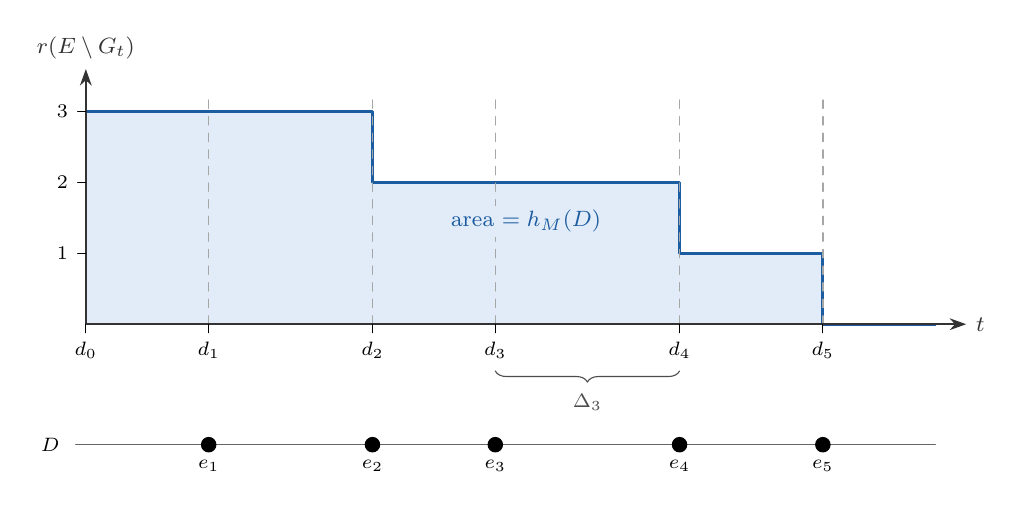
\begin{tikzpicture}[x=26mm,y=9mm]
    \fill[accl] (0,0) -- (0,3) -- (1.4,3) -- (1.4,2) -- (2.9,2)
      -- (2.9,1) -- (3.6,1) -- (3.6,0) -- cycle;
    \draw[line width=1pt,acc] (0,3) -- (1.4,3) -- (1.4,2) -- (2.9,2)
      -- (2.9,1) -- (3.6,1) -- (3.6,0) -- (4.15,0);
    \foreach \x/\k in {0.6/1,1.4/2,2.0/3,2.9/4,3.6/5}
      \draw[black!35,dashed,line width=0.5pt] (\x,0) -- (\x,3.25);
    \draw[axis] (0,0) -- (4.3,0) node[right,lab] {$t$};
    \draw[axis] (0,0) -- (0,3.6) node[above,lab] {$r(E\setminus G_t)$};
    \foreach \y in {1,2,3}
      \draw (0,\y) -- (-0.04,\y) node[left,slab] {$\y$};
    \foreach \x/\k in {0/0,0.6/1,1.4/2,2.0/3,2.9/4,3.6/5}
      \draw (\x,0) -- (\x,-0.12) node[below,slab] {$d_{\k}$};
    \draw[black!60] (-0.05,-1.7) -- (4.15,-1.7);
    \foreach \x/\k in {0.6/1,1.4/2,2.0/3,2.9/4,3.6/5} {
      \node[dotS] at (\x,-1.7) {};
      \node[slab,below=2pt] at (\x,-1.7) {$e_{\k}$};}
    \node[slab,anchor=east] at (-0.08,-1.7) {$D$};
    \draw[decorate,decoration={brace,amplitude=4pt,mirror},black!70]
      (2.0,-0.66) -- (2.9,-0.66) node[midway,below=5pt,slab] {$\Delta_3$};
    \node[lab,text=acc,fill=accl,inner sep=1.5pt] at (2.15,1.45) {area $=h_M(D)$};
  \end{tikzpicture}
  \caption{Lemma~\ref{lem:greedy} on five elements with $D_{e_i}=d_i$ and a rank-3
  matroid in which $e_3$ lies in the closure of $\{e_4,e_5\}$.  The step function
  is the rank of the elements above the threshold.  Its area,
  $0.6\cdot3+0.8\cdot3+0.6\cdot2+0.9\cdot2+0.7\cdot1=7.9$, is the weight of the
  greedy base $\{e_5,e_4,e_2\}$, and Theorem~\ref{thm:compiler} computes it one difference
  $\Delta_i$ at a time, without reading the order of the elements.}
  \label{fig:greedy}
\end{figure}

\begin{proof}[Proof of Theorem~\ref{thm:B}]
\emph{Step 1: $|a_j|\le2^{S}<2^{W-1}$.}  On inputs in $\{0,1\}$ the value $a_j$ of the $j$-th gate
is an integer.  Its arguments $a,b$ are sources or earlier gates, so
$|a|,|b|\le2^{j-1}$ by induction, and as $|a\pm b|\le2\max(|a|,|b|)$ and
$|\max(a,b)|\le\max(|a|,|b|)$,
\[
  |a_j|\le2\max(|a|,|b|)\le2^{j}\le2^{S}<2^{W-1}\qquad(W=S+2).
\]
So all values are exact in $W$-bit two's complement, where sums and differences
are exact and two's complement comparison is the comparison of integers.

\emph{Step 2: each gate with at most $15W+10$ Boolean gates.}  With full adders of eleven gates and $1=\neg0$, the
gadgets cost at most
\[
  a+b:\ 11W,\qquad a-b=a+\neg b+1:\ 12W+1,\qquad \max(a,b):\ 15W+10,
\]
where, with $c$ the carry out of $a+\neg b+1$,
\[
  \neg[a<b]=(a_{W-1}\oplus b_{W-1})\oplus c,\qquad
  \max(a,b)_i=\bigl([a<b]\wedge b_i\bigr)\vee\bigl(\neg[a<b]\wedge a_i\bigr).
\]

\emph{Step 3: $15S^{2}+40S$ gates in all.}  Each input bit becomes a $W$-bit number with high bits
$0$, and each of the $S$ gates its gadget, at most
\[
  S(15W+10)=S\bigl(15(S+2)+10\bigr)=15S^{2}+40S
\]
gates in all; by Step 1 the wires carry the values of the $(\max,+,-)$-circuit.

\emph{Step 4: $h_M(\mathbf 1_T)=r(T)$.}  For $T\subseteq E$,
\[
  h_M(\mathbf 1_T)=\max_{B}|B\cap T|=r(T),\qquad0\le r(T)\le2^{S}<2^{W-1},
\]
so the output bits are the binary digits of $r(T)$.
\end{proof}

\begin{corollary}
\label{cor:equiv}
Let $\STrop(h_M)$ be the least size of a $(\max,+,-)$-circuit that computes $h_M$
at every $w\in\R^{E}$, and $\Bool(r)$ the least size of a Boolean rank circuit of
$M$.
Then
\begin{align*}
  \STrop(h_M)&\le3m\,\Bool(r)+mL+9m^{2}+4m+4L+1,\\
  \Bool(r)&\le15\,\STrop(h_M)^{2}+40\,\STrop(h_M),
\end{align*}
and the second inequality holds also with the least size of a circuit that
computes $h_M$ on $\{0,1\}^{E}$ only.
\end{corollary}

\begin{corollary}
\label{cor:classes}
For the following matroids $M$ on $m$ elements, the function $h_M$ has a $(\max,+,-)$-circuit of polynomial size.
\begin{enumerate}
  \item A binary matroid represented by an $n\times m$ matrix over $\mathrm{GF}(2)$:
        it has a Boolean rank circuit of size
        $m(9n^{2}+5n)+11n\lceil\log_2(n+1)\rceil$, so $h_M$ has a $(\max,+,-)$-circuit of size at most $100(m+1)^{2}(n+1)^{2}$.
  \item A matroid represented by an $n\times m$ matrix over a finite field with $q$
        elements: it has a Boolean rank circuit of size
        $m(6q^{2}n^{2}+3qn^{2}+n^{2}+qn+6n+1)+11n\lceil\log_2(n+1)\rceil+1
        \le8q^{2}(m+1)(n+1)^{2}$, so $h_M$ has a $(\max,+,-)$-circuit of size at
        most $25q^{2}(m+1)^{2}(n+1)^{2}$.
  \item A matroid represented over $\mathbb Q$ by an $n\times m$ integer matrix whose
        entries have absolute value less than $2^{b}$: it has a Boolean rank circuit
        of size at most $2^{19}(m+1)(n+1)^{2}(n(n+b)+1)^{6}$, so $h_M$ has a $(\max,+,-)$-circuit of size at most $2^{21}(m+1)^{2}(n+1)^{2}(n(n+b)+1)^{6}$.
  \item The dual $M^{*}$ of a matroid $M$ with a Boolean rank circuit of size $s$:
        it has a Boolean rank circuit of size
        $s+m+1+11(m+1)\lceil\log_2(m+1)\rceil$.
  \item The cycle matroid $M(G)$ of a multigraph $G$ with $n$ vertices and $m$
        edges, whose independent sets are the edge sets containing no cycle, and its
        dual: $h_{M(G)}$ and $h_{M(G)^{*}}$ have $(\max,+,-)$-circuits of sizes at
        most $100(m+1)^{2}(n+1)^{2}$ and $100(m+1)^{2}((n+1)^{2}+m+1)$.
\end{enumerate}
\end{corollary}

\begin{proof}
\emph{Item 1.}  The circuit keeps $n$ slots, slot $p$ holding an occupancy bit
$f_p$ and a vector $b_p\in\mathrm{GF}(2)^{n}$, all empty at the start, and
processes column $e$ with its input bit $x_e$ by
\begin{align*}
  &v_i\leftarrow x_e\wedge A_{ie}\qquad(i\le n),\\
  &v_i\leftarrow v_i\oplus\bigl((v_p\wedge f_p)\wedge b_{p,i}\bigr)\qquad(p=1,\ldots,n,\ i\le n),\\
  &\ell_p=v_p\wedge\neg\textstyle\bigvee_{p'<p}v_{p'},\qquad f_p\leftarrow f_p\vee\ell_p,\qquad
   b_{p,i}\leftarrow(\ell_p\wedge v_i)\vee(\neg\ell_p\wedge b_{p,i}).
\end{align*}
Let $P=\{p:f_p=1\}$.  By induction on the columns, after column $e$ every $b_p$ with
$p\in P$ has $b_{p,i}=0$ for $i<p$ and $b_{p,p}=1$, and
\[
  \operatorname{span}\{b_p:p\in P\}=\operatorname{span}\{A_{\cdot e'}:e'\le e,\ x_{e'}=1\},
\]
since after the second line
\[
  v\in x_eA_{\cdot e}+\operatorname{span}\{b_p:p\in P\},\qquad v_p=0\quad(p\in P),
\]
and the third line stores $v$, if $v\ne0$, in the slot $\min\{i:v_i=1\}\notin P$.
Vectors with leading $1$s in distinct positions are independent, so at the end
the number of occupied slots, $|P|=\dim\operatorname{span}\{A_{\cdot e}:x_e=1\}$, is
the rank of the input set, and the size is
\[
  m(9n^{2}+5n)+11n\lceil\log_2(n+1)\rceil,
\]
the last term for counting the occupied slots.  Theorem~\ref{thm:A} with $k\le n$
gives the second bound.

\emph{Item 2.}  The same elimination runs over $\mathrm{GF}(q)$, an element
being carried by $q$ wires of which exactly one is true: a binary field operation
costs $2q^{2}$ gates, inversion none, masking by a bit $q$ and selection $3q$.
The column step
\[
  \begin{gathered}
  v\leftarrow x_eA_{\cdot e},\qquad v\leftarrow v-[f_p]\,v_p\,b_p\ \ (p=1,\ldots,n),\\
  f_p\leftarrow f_p\vee\ell_p,\qquad
  b_p\leftarrow\begin{cases}v_p^{-1}v&\text{if }\ell_p,\\b_p&\text{otherwise}\end{cases}
  \end{gathered}
\]
costs $6q^{2}n^{2}+3qn^{2}+n^{2}+qn+6n+1$ gates and keeps the invariant of item 1
with leading entries $1$.  Counting costs $11n\lceil\log_2(n+1)\rceil$ gates and
the constant $1$ one gate, and Theorem~\ref{thm:A}, applied to the exact count with
$k\le n$ and $q\ge2$, gives the second bound.

\emph{Item 3.}  Put $d=2n(n+b)+1$ and $N=2^{2\lceil\log_2(d+2)\rceil+1}$, so that
$N\le8(d+1)^{2}$ and $(N+1)N^{d}<2^{N}$.  For $S\subseteq E$, with $A_S$ the
matrix of the columns in $S$, and a prime $p$,
$\operatorname{rk}_{\mathrm{GF}(p)}A_S\le\operatorname{rk}_{\mathbb Q}A_S$, since a
rational dependence scales to an integer one with coprime coefficients, which
stays nontrivial modulo $p$.  Conversely let $I$ be a basis of $S$ over
$\mathbb Q$ and $g=\det(A_I^{\mathsf T}A_I)$.  By Hadamard's inequality,
\[
  0<|g|\le\prod_{j\in I}\|A_{\cdot j}\|_2^{2}\le(n\,4^{b})^{n}\le2^{2n(n+b)}<2^{d}.
\]
If every prime $p\le N$ divided $g$, then $2^{\pi(N)}\le\prod_{p\le N}p\le|g|<2^{d}$,
and since $\binom Nj$ divides
$\operatorname{lcm}(1,\ldots,N)=\prod_{p\le N}p^{\lfloor\log_pN\rfloor}$,
\[
  2^{N}=\sum_{j=0}^{N}\binom Nj\le(N+1)\operatorname{lcm}(1,\ldots,N)
  \le(N+1)N^{\pi(N)}<(N+1)N^{d}<2^{N}.
\]
So some prime $p\le N$ does not divide $g$, $A_I$ stays independent modulo $p$, and
\[
  \operatorname{rk}_{\mathbb Q}A_S=|I|\le\operatorname{rk}_{\mathrm{GF}(p)}A_S
  \le\max_{p'\le N\text{ prime}}\operatorname{rk}_{\mathrm{GF}(p')}A_S\le\operatorname{rk}_{\mathbb Q}A_S,
\]
so the maximum is $\operatorname{rk}_{\mathbb Q}A_S$.
The circuits of item 2 for all primes $p\le N$ with a running maximum, by the
two's complement comparison of the proof of Theorem~\ref{thm:B}, have at most
$2^{19}(m+1)(n+1)^{2}(n(n+b)+1)^{6}$ gates.

\emph{Item 4.}  With $W=\lceil\log_2(m+1)\rceil$,
\[
  r^{*}(S)=|S|+r(E\setminus S)-r(E)
  \equiv\bigl(2^{W}-(r(E)\bmod2^{W})\bigr)+\sum_{e\in S}1+r(E\setminus S)\pmod{2^{W}},
\]
computed by a $W$-bit counter started at the constant and fed the $m$ input bits
($11Wm$ gates), a ripple-carry adder for $r(E\setminus S)$ ($11W$ gates), $m$
negations, the given circuit and one gate for the constant $1$.  Since
$0\le r^{*}(S)\le m<2^{W}$, the result is $r^{*}(S)$, at
$s+m+1+11(m+1)W$ gates.

\emph{Item 5.}  Let $\chi_e\in\mathrm{GF}(2)^{V(G)}$ be the column of edge $e$ in
the vertex-edge incidence matrix.  For a nonempty edge set $F$,
\[
  \sum_{e\in F}\chi_e=0\iff\deg_F(x)\equiv0\pmod2\text{ for every vertex }x,
\]
which holds for a cycle.  Conversely a nonempty $F$ with even degrees contains a
cycle: a loop, or else the last vertex of a longest path in $F$ has a second edge
in $F$, which by maximality returns to the path.  Hence, for every edge set $F$,
\[
  \begin{aligned}
  (\chi_e)_{e\in F}\text{ is dependent over }\mathrm{GF}(2)
  &\iff\sum_{e\in F'}\chi_e=0\text{ for some nonempty }F'\subseteq F\\
  &\iff F\text{ contains a cycle},
  \end{aligned}
\]
so the matrix represents $M(G)$, and items 1 and 4 with
Theorem~\ref{thm:A} give the two bounds.
\end{proof}

More generally, a computation of time $T$ on inputs of a fixed length is
simulated by a Boolean circuit of size $O(T\log T)$~\cite{pippenger-fischer79}.
So every matroid whose rank is computed in time polynomial in $m$ and in the
length of a fixed description has a Boolean rank circuit, and by
Theorem~\ref{thm:A} a $(\max,+,-)$-circuit for $h_M$, of size polynomial in
these two quantities.  Corollary~\ref{cor:transversal} gives explicit sizes for
transversal matroids and gammoids.

\begin{corollary}
\label{cor:count}
For all large $m$, most matroids $M$ on $m$ labeled elements have no $(\max,+,-)$-circuit for $h_M$ of size less than $2^{m/2}/m^{2}$.
\end{corollary}

\begin{proof}
\emph{Step 1: at least $2^{2^{m}/(m(m+1))}$ matroids on $E$.}  Let $m\ge2$, $k=\lfloor m/2\rfloor$,
$E=\{0,\ldots,m-1\}$, and let $\mathcal H$ be a largest class of $k$-subsets of
$E$ under $X\mapsto\sum_{x\in X}x\bmod m$, so
$|\mathcal H|\ge\binom mk/m$~\cite{graham-sloane80}.  Distinct $X,Y\in\mathcal H$
satisfy $|X\cap Y|\le k-2$: otherwise $X\setminus Y=\{a\}$, $Y\setminus X=\{b\}$
and
\[
  a-b\equiv\sum_{x\in X}x-\sum_{y\in Y}y\equiv0\pmod m,
\]
so $a=b$.  For $H\subseteq\mathcal H$ let $\mathcal B_H=\binom Ek\setminus H$.  It
is nonempty: for $X\in H$, $a\in X$ and $b\notin X$, $|(X-a+b)\cap X|=k-1$, so
$X-a+b\notin H$.  It satisfies basis exchange: for
$B_1,B_2\in\mathcal B_H$ and $e\in B_1\setminus B_2$, either
$B_2\setminus B_1=\{f\}$ and $B_1-e+f=B_2$, or $B_2\setminus B_1\ni f_1\ne f_2$ and
\[
  \bigl|(B_1-e+f_1)\cap(B_1-e+f_2)\bigr|=k-1,
\]
so $B_1-e+f_1$ or $B_1-e+f_2$ lies in $\mathcal B_H$.  Distinct $H$ give distinct
matroids, and $\binom mk\ge2^{m}/(m+1)$ as the largest of $m+1$ coefficients with
sum $2^{m}$, so the number of matroids on $E$ is at least
\[
  2^{|\mathcal H|}\ge2^{\binom mk/m}\ge2^{2^{m}/(m(m+1))}.
\]
Knuth~\cite{knuth74} proves the stronger bound $2^{2^{m-\frac32\log_2m-O(1)}}$.

\emph{Step 2: at most $2^{O(2^{m}m^{-5/2})}$ of them have small circuits.}  Boolean circuits of size $s'$ on $m$ inputs
with at most $m$ outputs number $2^{O(s'\log(s'+m))}$, and each computes at most
one rank function.  If $h_M$ has a $(\max,+,-)$-circuit of size
$S<2^{m/2}/m^{2}$, Theorem~\ref{thm:B}, keeping the first $m$ output bits, gives a
Boolean rank circuit of size
\[
  s'\le15S^{2}+40S<\frac{15\cdot2^{m}}{m^{4}}+\frac{40\cdot2^{m/2}}{m^{2}}<\frac{2^{m}}{m^{7/2}}
\]
for large $m$, and
\[
  2^{O(s'\log(s'+m))}=2^{O(2^{m}m^{-5/2})}=o\bigl(2^{2^{m}/(m(m+1))}\bigr).\qedhere
\]
\end{proof}

\section{Rainbow bases}
\label{sec:rainbow}

\subsection{Setting and the Lagrangian}
\label{sec:lagr}

Throughout this section the rank function of $M$ is written $r_M$, as the letter
$r$ denotes a stage, and $E_Q=\bigcup_{b\in Q}R_b$ for $Q\subseteq[k]$.  For a
matroid $N$ on $E$ let $\nu(N)$ be the
largest size of a rainbow independent set of $N$, and let $\Av(N)$ be the set of
blocks missed by some rainbow independent set of size $\nu(N)$; we call these
blocks \emph{avoidable}.  These notions, and Lemmas~\ref{lem:avoidable}
and~\ref{lem:augment} below, apply with the same proofs to any partition of a
finite ground set into any number $k$ of blocks, and Section~\ref{sec:two} uses them
in that generality.  We assume that $M$ has a rainbow base; the algorithm that produces
the circuit checks this once by unweighted matroid intersection.

\begin{proposition}
\label{prop:star}
For every bipartite graph $H=(U,V,F)$ with $|U|=|V|=n$ there is a multigraph with
colored edges whose rainbow spanning trees are the perfect matchings of $H$, with
the same weights.  Its rainbow spanning tree polynomial is the permanent of the
biadjacency matrix of $H$ with variable entries.
\end{proposition}

\begin{proof}
\emph{Step 1: the multigraph on $\{z\}\cup V$.}  On the vertex set $\{z\}\cup V$ take, for each edge
$ij\in F$ with $i\in U$ and $j\in V$, an edge $zj$ of color $i$ and weight
$w_{ij}$ (Figure~\ref{fig:star}).

\emph{Step 2: $T_\pi$ is rainbow $\iff$ $\{\pi(j)j:j\in V\}$ is a perfect matching.}  Each $j\in V$ is adjacent only to $z$, so the
spanning trees are the sets $T_\pi$ containing, for each $j\in V$, the edge $zj$ of
color $\pi(j)$, where $\pi:V\to U$ and $\pi(j)j\in F$.  As $|U|=|V|$,
\[
  T_\pi\text{ rainbow}\iff\pi\text{ bijective}
  \iff\{\pi(j)j:j\in V\}\text{ is a perfect matching of }H,
\]
and $w(T_\pi)=\sum_{j\in V}w_{\pi(j)j}$ is the weight of this matching.  With
variable weights $x_{ij}$,
\[
  \sum_{T_\pi\text{ rainbow}}\ \prod_{j\in V}x_{\pi(j)j}
  =\sum_{\pi:V\to U\text{ bijective}}\ \prod_{j\in V}X_{\pi(j)j}=\operatorname{per}(X),
\]
where $X$ is the biadjacency matrix with $X_{ij}=x_{ij}$ on the edges and
$X_{ij}=0$ elsewhere, so that a bijection using a non-edge contributes $0$.
\end{proof}

\begin{figure}[t]
  \centering
  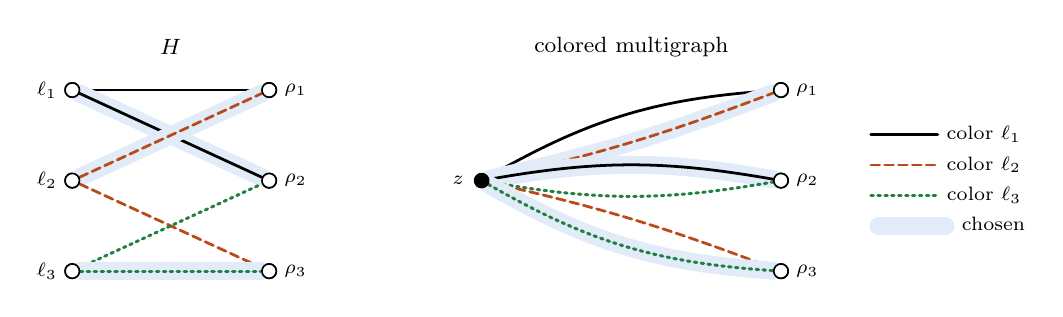
\begin{tikzpicture}[x=10mm,y=10mm]
    \definecolor{cgr}{RGB}{34,128,66}
    \tikzset{row1/.style={line width=1pt,black},
      row2/.style={line width=1pt,wrm,dash pattern=on 3.2pt off 1.8pt},
      row3/.style={line width=1.1pt,cgr,dash pattern=on 0.9pt off 1.6pt},
      pick/.style={preaction={draw,solid,accl,line width=6.5pt}}}
    \foreach \i/\y in {1/0,2/-1.15,3/-2.3} {
      \node[dotO] (L\i) at (0,\y) {};
      \node[slab,left=2pt] at (L\i) {$\ell_{\i}$};
      \node[dotO] (R\i) at (2.5,\y) {};
      \node[slab,right=2pt] at (R\i) {$\rho_{\i}$};}
    \draw[row1] (L1) -- (R1);
    \draw[row1,pick] (L1) -- (R2);
    \draw[row2,pick] (L2) -- (R1);
    \draw[row2] (L2) -- (R3);
    \draw[row3] (L3) -- (R2);
    \draw[row3,pick] (L3) -- (R3);
    \foreach \i in {1,2,3} {\node[dotO] at (L\i) {}; \node[dotO] at (R\i) {};}
    \node[lab] at (1.25,0.55) {$H$};
    \node[dotS] (z) at (5.2,-1.15) {};
    \node[slab,left=3pt] at (z) {$z$};
    \foreach \j/\y in {1/0,2/-1.15,3/-2.3} {
      \node[dotO] (S\j) at (9.0,\y) {};
      \node[slab,right=2pt] at (S\j) {$\rho_{\j}$};}
    \draw[row1] (z) to[bend left=13] (S1);
    \draw[row2,pick] (z) to[bend right=4] (S1);
    \draw[row1,pick] (z) to[bend left=10] (S2);
    \draw[row3] (z) to[bend right=10] (S2);
    \draw[row2] (z) to[bend left=4] (S3);
    \draw[row3,pick] (z) to[bend right=13] (S3);
    \foreach \j in {1,2,3} \node[dotO] at (S\j) {};
    \node[dotS] at (z) {};
    \node[lab] at (7.1,0.55) {colored multigraph};
    \node[slab,align=left,anchor=west] at (10.0,-1.15)
      {\tikz[baseline=-0.6ex]\draw[row1](0,0)--(0.85,0);\ color $\ell_1$\\[3pt]
       \tikz[baseline=-0.6ex]\draw[row2](0,0)--(0.85,0);\ color $\ell_2$\\[3pt]
       \tikz[baseline=-0.6ex]\draw[row3](0,0)--(0.85,0);\ color $\ell_3$\\[3pt]
       \tikz[baseline=-0.6ex]\draw[accl,line width=6.5pt](0,0)--(0.85,0);\ chosen};
  \end{tikzpicture}
  \caption{Proposition~\ref{prop:star}.  Each edge $\ell_i\rho_j$ of $H$ becomes an
  edge $z\rho_j$ of color $\ell_i$.  A spanning tree picks one edge at every
  $\rho_j$; it is rainbow exactly when the picked edges form a perfect matching,
  highlighted on both sides.}
  \label{fig:star}
\end{figure}

For $y\in\R^{k}$ let $y_{\blk}\in\R^{E}$ have the entries $y_{\blk(e)}$.  For
$p\in\R^{k}$ the shifted weights are $v=w-p_{\blk}$ and the Lagrangian is
$\Psi(p)=\sum_{b=1}^{k}p_b+\beta_M(v)$.  Let
\[
  \nu_0=\nu(M^{v}),\qquad S_0=\Av(M^{v}).
\]
Since rainbow independent sets of $M^{v}$ extend to minimum bases of $v$, and a
minimum base meeting $j$ blocks contains a rainbow set of size $j$, $\nu_0$ is the
largest number of blocks met by a minimum base of $v$, and $S_0$ is the set of
blocks missed by some minimum base meeting $\nu_0$ blocks.

\begin{lemma}
\label{lem:duality}
$\Psi(p)\le\Opt(w)$ for every $p$, and $\Psi(p)=\Opt(w)$ whenever $\nu_0=k$.
\end{lemma}

\begin{proof}
\emph{Step 1: $\Psi(p)\le\Opt(w)$.}  A rainbow base $B$ meets every block once, so
\[
  w(B)=\sum_{e\in B}\bigl(v_e+p_{\blk(e)}\bigr)=\sum_{b=1}^{k}p_b+v(B)
  \ge\sum_{b=1}^{k}p_b+\beta_M(v)=\Psi(p).
\]

\emph{Step 2: $\Psi(p)=\Opt(w)$ if $\nu_0=k$.}  If $\nu_0=k$, a rainbow independent set of
$M^{v}$ of size $k$ is a rainbow base $B$ with $v(B)=\beta_M(v)$, and
\[
  \Opt(w)\le w(B)=\sum_{b=1}^{k}p_b+\beta_M(v)=\Psi(p)\le\Opt(w).\qedhere
\]
\end{proof}

\subsection{Possibly optimal bases}
\label{sec:pos}

\begin{definition}
\label{def:theta}
For a base $B$ let
$\theta(B)=\max\bigl(\{0\}\cup\{v_f-v_e:e\notin B,\ f\in C(B,e)\}\bigr)$, the
largest gain of a single exchange, and let
$\Pos_t=\{B\in\Bases(M):\theta(B)\le t\}$ for $t\ge0$.
\end{definition}

\begin{proposition}
\label{prop:pos}
For a base $B$ and $t\ge0$ the following are equivalent.
\begin{enumerate}
  \item $\theta(B)\le t$.
  \item $B$ is a minimum base for $v-t\mathbf 1_B$.
  \item $v(B)-v(B')\le t\,|B\setminus B'|$ for every base $B'$.
  \item $e\in\cl\bigl(B\cap\{g:v_g\le v_e+t\}\bigr)$ for every $e\in E$.
  \item $B$ is a minimum base for some $u$ with $\|u-v\|_\infty\le t/2$.
\end{enumerate}
\end{proposition}

\begin{proof}
Throughout, $e\notin B$ and $f\in C(B,e)-e\subseteq B$, and $u=v-t\mathbf 1_B$.

\emph{(1)$\Leftrightarrow$(2).}  By Lemma~\ref{lem:minbases}(1),
\[
  \text{(2)}\iff u_f-u_e=v_f-v_e-t\le0\ \text{for all }e\notin B,\ f\in C(B,e)-e\iff\theta(B)\le t.
\]

\emph{(2)$\Rightarrow$(3).}  For a base $B'$, $u(B)\le u(B')$ gives
\[
  v(B)-v(B')\le t\bigl(|B|-|B\cap B'|\bigr)=t\,|B\setminus B'|.
\]

\emph{(3)$\Rightarrow$(1).}  For the base $B'=B-f+e$,
$v_f-v_e=v(B)-v(B')\le t\,|B\setminus B'|=t$.

\emph{(1)$\Leftrightarrow$(4).}  For $e\in B$, (4) holds as
$e\in B\cap\{g:v_g\le v_e+t\}$, and for $e\notin B$,
\[
  e\in\cl\bigl(B\cap\{g:v_g\le v_e+t\}\bigr)\iff C(B,e)-e\subseteq\{g:v_g\le v_e+t\}.
\]

\emph{(2)$\Rightarrow$(5).}  The weight $u+\tfrac t2\mathbf 1$ has the minimum
bases of $u$, and
$\|u+\tfrac t2\mathbf 1-v\|_\infty=\|\tfrac t2\mathbf 1-t\mathbf 1_B\|_\infty=\tfrac t2$.

\emph{(5)$\Rightarrow$(1).}  If $B$ is minimum for $u'$ with
$\|u'-v\|_\infty\le t/2$, then $u'_f\le u'_e$ by Lemma~\ref{lem:minbases}(1), and
\[
  v_f-v_e\le\bigl(u'_f+\tfrac t2\bigr)-\bigl(u'_e-\tfrac t2\bigr)\le t.\qedhere
\]
\end{proof}

So $\Pos_t$ is the family of bases that are possibly optimal for the interval
weights $[v-\tfrac t2,v+\tfrac t2]$~\cite{kasperski08}.  It grows with $t$,
equals $\Bases(M^{v})$ at $t=0$, and equals $\Bases(M)$ for
$t\ge\max v-\min v$.

\begin{lemma}
\label{lem:path}
If $y\in[0,t]^{k}$, every minimum base of $v-y_{\blk}$ lies in $\Pos_t$.
\end{lemma}

\begin{proof}
Let $B$ be a minimum base of $v-y_{\blk}$, $e\notin B$ and $f\in C(B,e)$.  By
Lemma~\ref{lem:minbases}(1), $v_f-y_{\blk(f)}\le v_e-y_{\blk(e)}$, so
\[
  v_f-v_e\le y_{\blk(f)}-y_{\blk(e)}\le t,
\]
and $\theta(B)\le t$.
\end{proof}

\subsection{Two obstacles}
\label{sec:obstacles}

Two facts keep the family $\Pos_t$ from being used directly.

\begin{proposition}
\label{prop:notmatroid}
For $U_{2,4}$ on $\{a,b,c,d\}$ with $v=(0,1,2,3)$, $\Pos_2=\{ab,ac,ad,bc\}$,
which violates the basis exchange axiom.
\end{proposition}

\begin{proof}
\emph{Step 1: $\Pos_2=\{ab,ac,ad,bc\}$.}  In $U_{2,4}$, $C(B,e)=B+e$ for
$e\notin B$, so
\[
  \theta(B)=\max\Bigl(0,\ \max_{f\in B}v_f-\min_{e\notin B}v_e\Bigr),\qquad
  \bigl(\theta(ab),\theta(ac),\theta(ad),\theta(bc),\theta(bd),\theta(cd)\bigr)=(0,1,2,2,3,3).
\]

\emph{Step 2: $ad-a+b,\ ad-a+c\notin\Pos_2$.}  For $B_1=ad$, $B_2=bc$ and
$a\in B_1\setminus B_2$, both candidates $B_1-a+f$, $f\in B_2\setminus B_1$, have
$\theta(bd)=\theta(cd)=3>2$.
\end{proof}

\begin{proposition}
\label{prop:nphard}
Given a multigraph with colored edges, edge weights $v$ and $t\ge0$, deciding
whether $\Pos_t$ contains a rainbow spanning tree is NP-complete.
\end{proposition}

\begin{proof}
\emph{Step 1: the problem is in NP.}  For a rainbow spanning tree $T$,
$\theta(T)=\max\bigl(\{0\}\cup\{v_g-v_e:e\notin T,\ g\in C(T,e)\}\bigr)$ is
computed from the fundamental cycles in polynomial time.

\emph{Step 2: a reduction from rainbow path.}  Rainbow path is NP-complete~\cite{cfmy09}: given a graph $H$ with colored edges and vertices $a,b$, is there a
path from $a$ to $b$ with distinct colors?  Let $Q$ be the colors of $H$,
$q=|Q|$, and $h\ge q$ the number of vertices of $H$ (add isolated vertices if
needed).  On $V(H)\cup\{z,y\}$ take the edges of $H$ with weight $5$, an edge
$e^{*}=ab$ of weight $0$ and a new color $c^{*}$, an edge $f=ya$ of weight $0$ and
color $c^{*}$, and for every $x\in V(H)$ and every color in $Q\cup X$ an edge $zx$
of that color and weight $10$, where $X$ is a set of $h-q$ new colors
(Figure~\ref{fig:gadget}).  There are $h+2$ vertices and $h+1$ colors, so a
rainbow spanning tree uses every color once.  Take $t=5$.

\emph{Step 3: a rainbow $T$ with $\theta(T)\le5$ gives a rainbow path in $H$.}  Let $T$ be a rainbow spanning tree with
$\theta(T)\le5$.  As $f$ is the only edge at $y$ and has the color of $e^{*}$,
$f\in T$ and $e^{*}\notin T$.  Every edge $g$ of the path $P_T$ of $T$ from $a$
to $b$ lies in $C(T,e^{*})$, so
\[
  v_g=v_g-v_{e^{*}}\le\theta(T)\le5<10.
\]
So $P_T$ avoids $z$ and the leaf $y$, lies in $H$, and is rainbow since $T$ is.

\emph{Step 4: a rainbow path in $H$ gives a rainbow $T$ with $\theta(T)\le5$.}  Let $P$ be a rainbow path from $a$ to $b$
in $H$.  Let $T$ consist of $E(P)$, $f$, an edge $zx$ for each
$x\in V(H)\setminus V(P)$ and one edge $zx$ with $x\in V(P)$, these
$h-|E(P)|$ edges at $z$ taking the $h-|E(P)|$ colors of $Q\cup X$ not on $P$.
Then $T$ is a rainbow spanning tree with $C(T,e^{*})=P+e^{*}$ and edge weights at
most $10$, so
\[
  \theta(T)\le\max\bigl(\underbrace{5-0}_{e=e^{*}},\ \underbrace{10-5}_{e\in E(H)\setminus T},\
  \underbrace{10-10}_{e=zx\notin T}\bigr)=5.\qedhere
\]
\end{proof}

\begin{figure}[t]
  \centering
  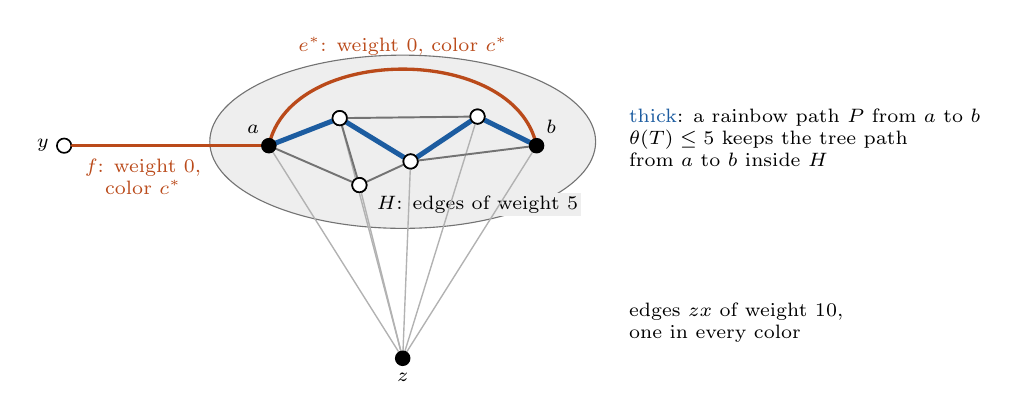
\begin{tikzpicture}[x=10mm,y=10mm]
    \draw[black!55,fill=grl] (2,0) ellipse (2.45 and 1.1);
    \node[slab,fill=grl,inner sep=1pt] at (2.95,-0.8) {$H$: edges of weight $5$};
    \node[dotO] (h1) at (1.2,0.3) {};
    \node[dotO] (h2) at (2.1,-0.25) {};
    \node[dotO] (h3) at (2.95,0.32) {};
    \node[dotO] (h4) at (1.45,-0.55) {};
    \coordinate (s) at (0.3,-0.05);
    \coordinate (t) at (3.7,-0.05);
    \foreach \v in {s,h4,h2,t,h1,h3}
      \draw[black!30,line width=0.5pt] (2,-2.75) -- (\v);
    \draw[black!55,line width=0.7pt] (s) -- (h4) -- (h2) (h1) -- (h3) (h2) -- (t)
      (h4) -- (h1);
    \draw[acc,line width=1.8pt] (s) -- (h1) -- (h2) -- (h3) -- (t);
    \draw[wrm,line width=1.2pt] (s) to[bend left=78]
      node[pos=0.5,above=1pt,slab,text=wrm] {$e^{*}$: weight $0$, color $c^{*}$} (t);
    \node[dotO] (y) at (-2.3,-0.05) {};
    \node[slab,left=2pt] at (y) {$y$};
    \draw[wrm,line width=1.2pt] (y) -- node[pos=0.36,below=1pt,slab,text=wrm,align=center]
      {$f$: weight $0$,\\color $c^{*}$} (s);
    \foreach \v in {h1,h2,h3,h4} \node[dotO] at (\v) {};
    \node[dotS] at (s) {};
    \node[dotS] at (t) {};
    \node[slab,above left=1pt and 0pt] at (s) {$a$};
    \node[slab,above right=1pt and 0pt] at (t) {$b$};
    \node[dotS] (z) at (2,-2.75) {};
    \node[slab,below=2pt] at (z) {$z$};
    \node[slab,align=left,anchor=west] at (4.75,-2.3)
      {edges $zx$ of weight $10$,\\one in every color};
    \node[slab,align=left,anchor=west] at (4.75,0.05)
      {\textcolor{acc}{thick}: a rainbow path $P$ from $a$ to $b$\\
       $\theta(T)\le5$ keeps the tree path\\from $a$ to $b$ inside $H$};
  \end{tikzpicture}
  \caption{The reduction of Proposition~\ref{prop:nphard}.  The bridge $f$ uses
  the color of $e^{*}$, so a rainbow spanning tree omits $e^{*}$, and the bound
  $\theta(T)\le5$ keeps the edges at $z$, of weight $10$, off the fundamental
  cycle of $e^{*}$.}
  \label{fig:gadget}
\end{figure}

\subsection{Admissible families and the update}
\label{sec:enlarge}

We therefore use matroids $N(t)$ with $\Pos_t\subseteq\Bases(N(t))$.

\begin{definition}
\label{def:admissible}
A family of matroids $N(t)$ on $E$, $t\ge0$, is \emph{admissible} if
\begin{enumerate}
  \item[(F1)] $N(0)=M^{v}$;
  \item[(F2)] every base of $N(t)$ is a base of $N(t')$ whenever $t\le t'$;
  \item[(F3)] $\Pos_t\subseteq\Bases(N(t))$ for every $t$;
  \item[(F4)] $N(t)$ has a rainbow base for all large $t$;
  \item[(F5)] there are levels $0=c_0<c_1<\cdots<c_q$ such that $N(t)$ is
        constant on each $[c_i,c_{i+1})$ and on $[c_q,\infty)$.
\end{enumerate}
\end{definition}

\begin{definition}
\label{def:update}
Let $r<k$ and $\nu_0\ge r$.  For an admissible family let
\[
  \tau=\min\{t:\nu(N(t))\ge r+1\},\quad
  \lambda_b=\min\{t:\text{some base of }N(t)\text{ meeting exactly }r\text{ blocks misses }b\},
\]
with $\lambda_b=\infty$ if there is none, and $a_b=(\tau-\lambda_b)_+=\max(\tau-\lambda_b,0)$.  The
vector $a$ is the update of stage $r$, and stage $r$ replaces $p$ by $p+a$ while
$\nu_0=r$.  If $\nu_0>r$, then $\tau=0$ and $a=0$.
\end{definition}

The minima exist: by (F2) independent sets of $N(t)$ stay independent in $N(t')$
for $t\le t'$, and $\nu(N(0))=\nu_0\ge r$ by (F1), so
\[
  r\le\nu(N(0))\le\nu(N(t))\le\nu(N(t'))\qquad(t\le t').
\]
Moreover $\nu(N(t))=k>r$ for large $t$ by (F4), and by (F5) both sets of levels are
unions of intervals $[c_i,c_{i+1})$ and $[c_q,\infty)$.  For $t<\tau$ we have
$\nu(N(t))=r$, a base of $N(t)$ meeting exactly $r$ blocks contains a rainbow
independent set of size $r$ missing the same blocks, and a rainbow independent
set of size $r$ extends to a base of $N(t)$ meeting no further block.  With (F2)
this gives, for $t<\tau$,
\[
  b\in\Av(N(t))\iff\text{some base of }N(t)\text{ meeting exactly }r\text{ blocks misses }b
  \iff\lambda_b\le t,
\]
and as $\mathbf 1[\nu(N(t))\le r]=\mathbf 1[t<\tau]$,
\begin{equation}
  a_b=(\tau-\lambda_b)_+=\int_0^{\tau}\mathbf 1[\lambda_b\le t]\,dt
  =\int_0^{\infty}\mathbf 1\bigl[\nu(N(t))\le r\bigr]\;\mathbf 1\bigl[b\in\Av(N(t))\bigr]\,dt.
  \label{eq:update-integral}
\end{equation}
Figure~\ref{fig:axis} draws the integrand.

\begin{figure}[t]
  \centering
  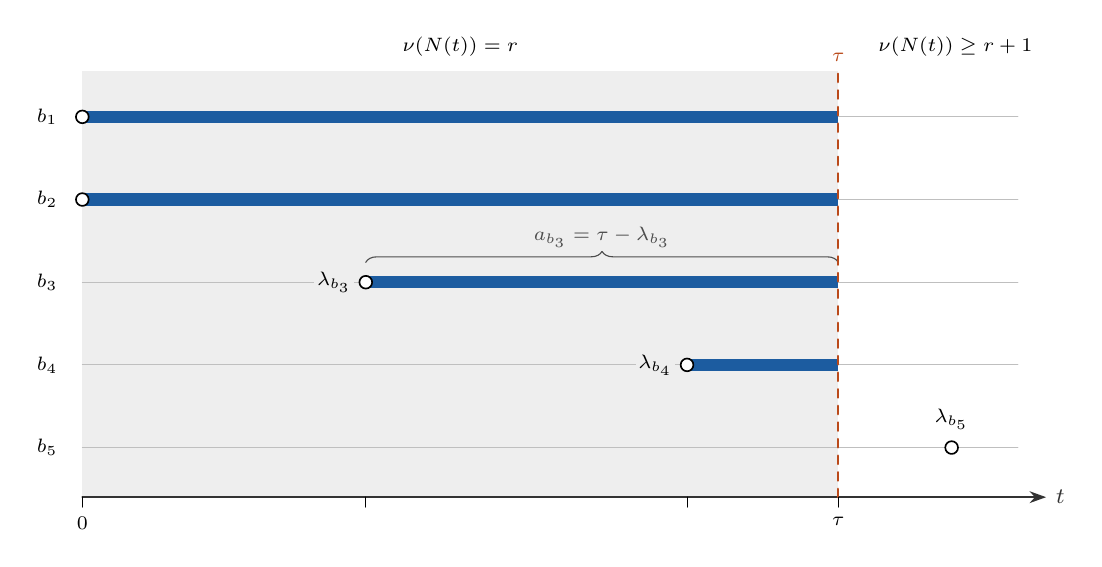
\begin{tikzpicture}[x=24mm,y=10.5mm]
    \fill[grl] (0,-0.6) rectangle (4,4.55);
    \draw[axis] (0,-0.6) -- (5.1,-0.6) node[right,lab] {$t$};
    \foreach \b/\lam/\y in {1/0/4,2/0/3,3/1.5/2,4/3.2/1} {
      \node[slab,anchor=east] at (-0.08,\y) {$b_{\b}$};
      \draw[black!25,line width=0.4pt] (0,\y) -- (4.95,\y);
      \draw[acc,line width=4.4pt,line cap=butt] (\lam,\y) -- (4,\y);
      \node[dotO,minimum size=4.6pt] at (\lam,\y) {};}
    \node[slab,anchor=east] at (-0.08,0) {$b_5$};
    \draw[black!25,line width=0.4pt] (0,0) -- (4.95,0);
    \node[dotO,minimum size=4.6pt] at (4.6,0) {};
    \node[slab,above=3pt] at (4.6,0) {$\lambda_{b_5}$};
    \node[slab,anchor=east,fill=grl,inner sep=1pt] at (1.44,2) {$\lambda_{b_3}$};
    \node[slab,anchor=east,fill=grl,inner sep=1pt] at (3.14,1) {$\lambda_{b_4}$};
    \draw[decorate,decoration={brace,amplitude=4pt},black!70]
      (1.5,2.24) -- (4,2.24) node[midway,above=4pt,slab,fill=grl,inner sep=1pt]
      {$a_{b_3}=\tau-\lambda_{b_3}$};
    \draw[wrm,dashed,line width=0.9pt] (4,-0.6) -- (4,4.55);
    \node[slab,text=wrm,anchor=south] at (4,4.55) {$\tau$};
    \node[slab] at (2,4.85) {$\nu(N(t))=r$};
    \node[slab] at (4.62,4.85) {$\nu(N(t))\ge r+1$};
    \foreach \x in {0,1.5,3.2,4}
      \draw (\x,-0.6) -- (\x,-0.72);
    \node[slab,below] at (0,-0.72) {$0$};
    \node[slab,below] at (4,-0.72) {$\tau$};
  \end{tikzpicture}
  \caption{The integrand of \eqref{eq:update-integral}.  Blocks $b_1,b_2\in S_0$
  are avoidable from level $0$ and receive $\tau$; block $b_3$ becomes avoidable
  at $\lambda_{b_3}$ and receives the length of the bar; $b_5$ has
  $\lambda_{b_5}>\tau$, where $\nu(N(t))\ge r+1$, and
  receives nothing.}
  \label{fig:axis}
\end{figure}

\begin{lemma}
\label{lem:avoidable}
Let $N$ be a matroid on $E$ and $\nu=\nu(N)$.
\begin{enumerate}
  \item $|Q|-r_N(E_Q)\le k-\nu$ for every $Q\subseteq[k]$.
  \item $|\Av(N)|-r_N(E_{\Av(N)})=k-\nu$.
  \item $\Av(N)\subseteq Q$ for every $Q$ attaining equality in item 1.
\end{enumerate}
\end{lemma}

\begin{proof}
\emph{Step 1: item 1.}  A rainbow independent set $J$ with $|J|=\nu$ satisfies
\[
  \nu=|J\cap E_Q|+|J\setminus E_Q|\le r_N(E_Q)+(k-|Q|).
\]

\emph{Step 2: $|A'|=(k-\nu)+|I\cap Z|$.}  Fix a rainbow independent set $I$ with
$|I|=\nu$, and let $D_I$ be the directed graph on $E$ with arcs
\[
  y\to x\ \ \text{if }I-x+y\text{ is independent},\qquad
  x\to y\ \ \text{if }\blk(y)=\blk(x)\qquad(x\in I,\ y\notin I),
\]
sources the $y\notin I$ in blocks missed by $I$, and sinks the $y\notin I$ with
$I+y$ independent.  As $I$ is maximum, no path leads from a source to a
sink~\cite{lawler75,schrijver03}.  Let $Z$ be the set reachable from the sources
and $A'=\{b:b\text{ missed by }I\}\cup\blk(I\cap Z)$, so
$|A'|=(k-\nu)+|I\cap Z|$.

\emph{Step 3: $A'\subseteq\Av(N)$.}  Blocks missed by $I$ are avoidable.  For
$x\in I\cap Z$ and a shortest path $y_0\to x_1\to y_1\to\cdots\to y_{j-1}\to x_j=x$
from a source $y_0$, the arcs give $\blk(y_i)=\blk(x_i)$ for $1\le i<j$, and
$\blk(y_0)\notin\blk(I)$, so $J=I-\{x_1,\ldots,x_j\}+\{y_0,\ldots,y_{j-1}\}$ has
\[
  |J|=\nu,\qquad\blk(J)=\bigl(\blk(I)-\blk(x)\bigr)+\blk(y_0),\qquad|\blk(J)|=\nu.
\]
Hence $J$ is rainbow and misses $\blk(x)$, and it is independent by the exchange
lemma for shortest paths~\cite{schrijver03}.

\emph{Step 4: $r_N(E_{A'})\le|I\cap Z|$.}  Let $y\in E_{A'}\setminus I$.  Either
$y$ is a source or $x\to y$ for some $x\in I\cap Z$, so $y\in Z$ is not a sink,
and $I+y$ contains a circuit $C_y$.  For $x'\in C_y-y$,
\[
  I-x'+y\text{ independent}\ \Rightarrow\ y\to x'\ \Rightarrow\ x'\in I\cap Z,
\]
so $y\in\cl_N(C_y-y)\subseteq\cl_N(I\cap Z)$.  As $I$ is rainbow and misses the
blocks of $A'$ outside $\blk(I\cap Z)$, $I\cap E_{A'}=I\cap Z$, and
\[
  E_{A'}\subseteq\cl_N(I\cap Z),\qquad r_N(E_{A'})\le|I\cap Z|.
\]

\emph{Step 5: item 3.}  Let $Q$ attain equality in item 1, and let
$b\in\Av(N)\setminus Q$ be missed by a rainbow independent $J$ with $|J|=\nu$.
As $J\setminus E_Q$ is rainbow and avoids the blocks of $Q+b$,
\[
  k-|Q|=\nu-|Q|+(k-\nu)=\nu-r_N(E_Q)\le\nu-|J\cap E_Q|=|J\setminus E_Q|\le k-|Q|-1,
\]
a contradiction.

\emph{Step 6: item 2.}  By item 1 and Steps 2 and 4,
\[
  k-\nu\ge|A'|-r_N(E_{A'})\ge(k-\nu)+|I\cap Z|-|I\cap Z|=k-\nu,
\]
so $A'$ attains equality, $\Av(N)\subseteq A'$ by Step 5, and $A'=\Av(N)$ by
Step 3.
\end{proof}

\begin{theorem}[Validity]
\label{thm:validity}
Let $\nu_0=r<k$, let $N(t)$ be admissible, and let $a$ be its update.  Then
\begin{enumerate}
  \item $\Psi(p+a)=\Psi(p)+(k-r)\tau$;
  \item every base of $M^{v}$ meeting $r$ blocks is a minimum base of
        $v-a_{\blk}$; in particular $\nu_0$ does not decrease.
\end{enumerate}
\end{theorem}

\begin{proof}
\emph{Step 1: $\varphi(t)=\Psi(p)+\int_0^{t}\varphi'(\sigma^{+})\,d\sigma$.}  For $t\in[0,\tau]$ put $a(t)_b=(t-\lambda_b)_+\in[0,t]$,
$v(t)=v-a(t)_{\blk}$ and $\varphi(t)=\Psi(p+a(t))$, so $a(0)=0$ and $a(\tau)=a$.
As a minimum of finitely many continuous piecewise linear functions of $t$,
$\varphi$ is continuous and piecewise linear, and
\[
  \varphi(t)-\varphi(0)=\int_0^{t}\varphi'(\sigma^{+})\,d\sigma.
\]

\emph{Step 2: $\varphi'(t^{+})=|S_t|-\max_{B\in\Bases(M^{v(t)})}|B\cap E_{S_t}|$.}  Let $S_t=\{b:\lambda_b\le t\}$.  For small
$h>0$, $a(t+h)=a(t)+h\mathbf 1_{S_t}$, and the minimum bases of
$v(t)-h\mathbf 1_{E_{S_t}}$ are the minimum bases of $v(t)$ with the most elements
in $E_{S_t}$.  Hence
\[
  \begin{aligned}
  \varphi'(t^{+})&=|S_t|+\frac{d}{dh}\,\beta_M\bigl(v(t)-h\mathbf 1_{E_{S_t}}\bigr)\Big|_{h=0^{+}}\\
  &=|S_t|-\max\bigl\{|B\cap E_{S_t}|:B\in\Bases(M^{v(t)})\bigr\}.
  \end{aligned}
\]

\emph{Step 3: $\varphi(t)\ge\Psi(p)+(k-r)t$.}  Let $t<\tau$.  By Lemma~\ref{lem:path} with
$y=a(t)$ and by (F3),
\[
  \Bases(M^{v(t)})\subseteq\Pos_t\subseteq\Bases(N(t)),
\]
and $\nu(N(t))=r$, $S_t=\Av(N(t))$ by the paragraph after
Definition~\ref{def:update}.  So Lemma~\ref{lem:avoidable}(2) gives, for every
$B\in\Bases(M^{v(t)})$,
\[
  |B\cap E_{S_t}|\le r_{N(t)}(E_{S_t})=|S_t|-(k-r),
\]
hence $\varphi'(t^{+})\ge k-r$ by Step 2, and by Step 1
\[
  \varphi(t)=\Psi(p)+\int_0^{t}\varphi'(\sigma^{+})\,d\sigma\ge\Psi(p)+(k-r)t\qquad(t\in[0,\tau]).
\]

\emph{Step 4: $\varphi(t)\le\Psi(p)+(k-r)t$.}  Let $B^{*}$ be a base of $M^{v}$ meeting exactly $r$
blocks.  Its $k-r$ missed blocks lie in $S_0\subseteq S_t$, as $\lambda_b=0$ on
$S_0$, and $B^{*}\in\Bases(N(t))$ by (F1) and (F2), so for $t<\tau$
\[
  |S_t|-(k-r)\le|B^{*}\cap E_{S_t}|\le r_{N(t)}(E_{S_t})=|S_t|-(k-r).
\]
Hence $v(t)(B^{*})+\sum_ba(t)_b$ has right derivative
$-(|S_t|-(k-r))+|S_t|=k-r$, so
$v(t)(B^{*})=\beta_M(v)-\sum_ba(t)_b+(k-r)t$, and
\[
  \varphi(t)\le\sum_{b=1}^{k}\bigl(p_b+a(t)_b\bigr)+v(t)(B^{*})
  =\sum_{b=1}^{k}p_b+\beta_M(v)+(k-r)t=\Psi(p)+(k-r)t.
\]

\emph{Step 5: items 1 and 2.}  By Steps 3 and 4, for $t\in[0,\tau]$,
\[
  \varphi(t)=\Psi(p)+(k-r)t,\qquad v(t)(B^{*})=\beta_M(v(t)).
\]
At $t=\tau$ these are items 1 and 2, and $\nu_0$ does not decrease since $B^{*}$
meets $r$ blocks.
\end{proof}

\begin{figure}[t]
  \centering
  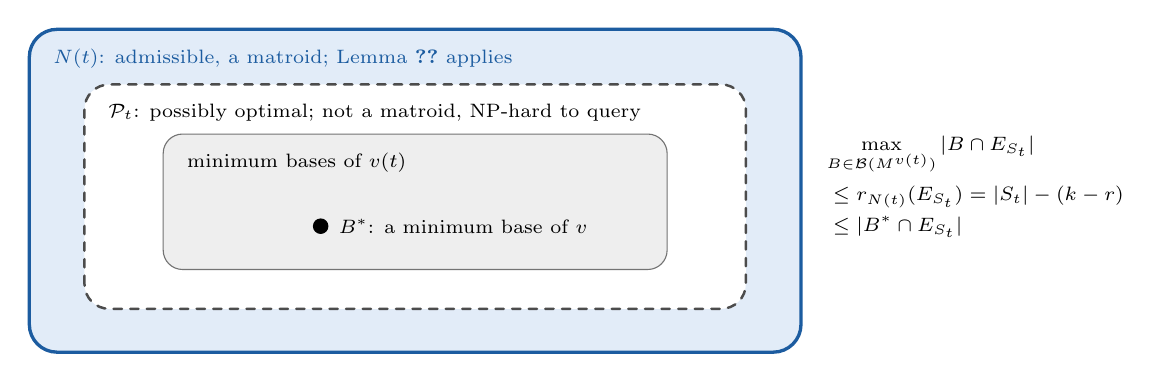
\begin{tikzpicture}[x=10mm,y=10mm]
    \draw[acc,line width=1.2pt,rounded corners=10pt,fill=accl]
      (-4.9,-2.05) rectangle (4.9,2.05);
    \draw[black!70,dashed,line width=0.9pt,rounded corners=9pt,fill=white]
      (-4.2,-1.5) rectangle (4.2,1.35);
    \draw[black!55,rounded corners=7pt,fill=grl] (-3.2,-1.0) rectangle (3.2,0.72);
    \node[slab,text=acc,anchor=north west] at (-4.72,1.92)
      {$N(t)$: admissible, a matroid; Lemma~\ref{lem:avoidable} applies};
    \node[slab,anchor=north west] at (-4.02,1.23)
      {$\Pos_t$: possibly optimal; not a matroid, NP-hard to query};
    \node[slab,anchor=north west] at (-3.02,0.6) {minimum bases of $v(t)$};
    \node[dotS] (bs) at (-1.2,-0.45) {};
    \node[slab,right=3pt] at (bs) {$B^{*}$: a minimum base of $v$};
    \node[slab,align=left,anchor=west] at (5.1,0.05)
      {$\displaystyle\max_{B\in\Bases(M^{v(t)})}|B\cap E_{S_t}|$\\[3pt]
       ${}\le r_{N(t)}(E_{S_t})=|S_t|-(k-r)$\\[3pt]
       ${}\le|B^{*}\cap E_{S_t}|$};
  \end{tikzpicture}
  \caption{The two bounds in the proof of Theorem~\ref{thm:validity}.  Every
  minimum base along the update path is possibly optimal (Lemma~\ref{lem:path}),
  hence a base of the matroid $N(t)$, whose rank bounds how many raised elements
  it holds; the base $B^{*}$ attains the bound, so it stays optimal and the
  rate stays $k-r$.  The middle family is never computed.}
  \label{fig:sandwich}
\end{figure}

\subsection{Single linkage on possibly optimal elements}
\label{sec:posl}

\begin{definition}
\label{def:posl}
For $t\ge0$ let
\[
  \PO_t=\bigl\{f\in E:f\notin\cl\{g:v_g<v_f-t\}\bigr\}.
\]
In each connected component $K$ of $M$, link $x,y\in\PO_t\cap K$ when
$|v_x-v_y|\le t$, and call the classes of the transitive closure of this relation
the \emph{clusters} of $K$ at scale $t$.  Each cluster is an interval of the
sorted values of $\PO_t\cap K$ in which consecutive values differ by at most $t$,
and consecutive values in different clusters differ by more than $t$.  So the
clusters of $K$ are ordered: every value of a cluster lies more than $t$ below
every value of the next one.  For $e\in\PO_t$ let $u_t(e)$ be the position of the
cluster of $e$ in this order, $1$ for the lowest cluster of its component, let
$u_t(e)=m+1$ for $e\notin\PO_t$, and let $N(t)=M^{u_t}$.  We call $N$ the \emph{PO-SL} family, for single linkage
on possibly optimal elements.
\end{definition}

By Lemma~\ref{lem:minbases}(4), $N(t)$ depends only on the comparisons of $u_t$
within components.  The inequalities matter: $\PO_t$
uses a strict inequality and the linkage a non-strict one
(Figure~\ref{fig:posl}).  With $v_g\le v_f-t$ in $\PO_t$, property (F1)
fails already for $U_{1,3}$ and $v=(0,0,1)$, and with $|v_x-v_y|<t$ in the
linkage, the two elements of value $0$ there form two clusters at scale $0$ that
are not ordered.  Write $\mathcal G_t=\{(e,f)\in E\times E:v_f-v_e\le t\}$.

\begin{figure}[t]
  \centering
  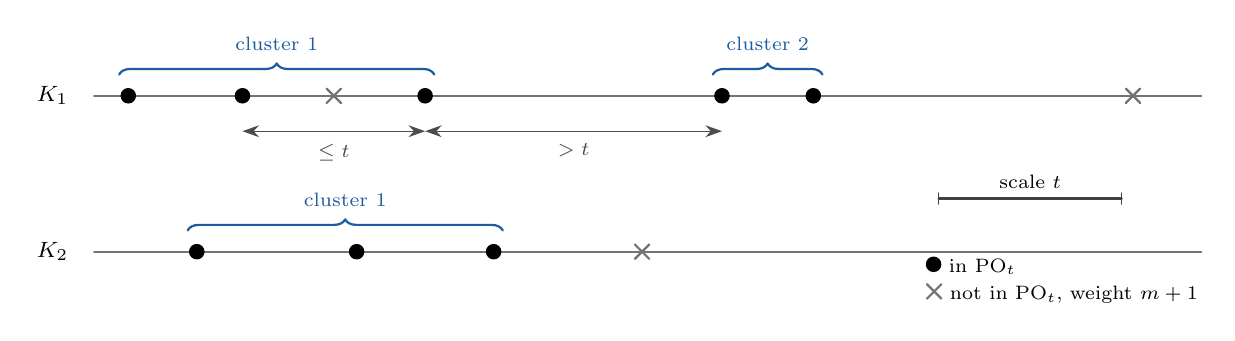
\begin{tikzpicture}[x=29mm,y=9mm]
    \foreach \y/\n in {0/K_1,-2.2/K_2} {
      \draw[black!55,line width=0.6pt] (-0.15,\y) -- (4.7,\y);
      \node[lab,anchor=east] at (-0.22,\y) {$\n$};}
    \foreach \x in {0,0.5,1.3,2.6,3.0}
      \node[dotS] at (\x,0) {};
    \node[dotX] at (0.9,0) {};
    \node[dotX] at (4.4,0) {};
    \draw[decorate,decoration={brace,amplitude=4pt},acc,line width=0.8pt]
      (-0.04,0.3) -- (1.34,0.3) node[midway,above=5pt,slab,text=acc] {cluster 1};
    \draw[decorate,decoration={brace,amplitude=4pt},acc,line width=0.8pt]
      (2.56,0.3) -- (3.04,0.3) node[midway,above=5pt,slab,text=acc] {cluster 2};
    \draw[<->,black!70,line width=0.5pt] (0.5,-0.5) -- (1.3,-0.5)
      node[midway,below=1pt,slab] {$\le t$};
    \draw[<->,black!70,line width=0.5pt] (1.3,-0.5) -- (2.6,-0.5)
      node[midway,below=1pt,slab] {$>t$};
    \foreach \x in {0.3,1.0,1.6}
      \node[dotS] at (\x,-2.2) {};
    \node[dotX] at (2.25,-2.2) {};
    \draw[decorate,decoration={brace,amplitude=4pt},acc,line width=0.8pt]
      (0.26,-1.9) -- (1.64,-1.9) node[midway,above=5pt,slab,text=acc] {cluster 1};
    \draw[black!75,line width=0.9pt] (3.55,-1.45) -- (4.35,-1.45);
    \draw[black!75] (3.55,-1.53) -- (3.55,-1.37) (4.35,-1.53) -- (4.35,-1.37);
    \node[slab,above] at (3.95,-1.45) {scale $t$};
    \node[slab,align=left,anchor=west] at (3.45,-2.6)
      {\tikz\node[dotS]{};\ in $\PO_t$\\[2pt]
       \tikz\node[dotX]{};\ not in $\PO_t$, weight $m+1$};
  \end{tikzpicture}
  \caption{Definition~\ref{def:posl} on two components.  Filled dots are
  possibly optimal, crosses are not and receive the top weight $m+1$.  Within a
  component, clusters are chains of steps of length at most $t$; the cross
  between two members of cluster 1 does not break the chain, and the clusters of
  different components are never compared.}
  \label{fig:posl}
\end{figure}

\begin{proposition}
\label{prop:posl}
For every $v$, the family $N(t)$ of Definition~\ref{def:posl}
satisfies (F1)--(F5) with levels $\{0\}\cup\{|v_e-v_f|:e,f\in E\}$.  It is
determined by $\mathcal G_t$.
\end{proposition}

\begin{proof}
\emph{Step 1: (F1).}  Every minimum base $B$ of $v$ lies in $\PO_0$: for $f\in B$,
Lemma~\ref{lem:minbases}(2) gives $\cl\{g:v_g<v_f\}=\cl(B\cap\{v<v_f\})\subseteq\cl(B-f)$,
which misses $f$.  At scale $0$ clusters are classes of equal values, so within a
component
\[
  u_0(x)\le u_0(y)\iff v_x\le v_y\qquad(x,y\in\PO_0).
\]
If $B$ is minimum for $v$, then $B\subseteq\PO_0$, and for $e\notin B$ and
$f\in C(B,e)$, where $v_f\le v_e$ by Lemma~\ref{lem:minbases}(1),
\[
  u_0(f)\le u_0(e)\quad\text{since}\quad
  \begin{cases}
    u_0(e)=m+1,&e\notin\PO_0,\\
    v_f\le v_e,&e\in\PO_0,
  \end{cases}
\]
so $B$ is minimum for $u_0$ by Lemma~\ref{lem:minbases}(1).  Conversely let $B$ be
minimum for $u_0$, $c\in\R$, and $K_x$ the component of $x$.  For
$x\in\PO_0\setminus B$ with $v_x\le c$, Lemma~\ref{lem:minbases}(1) gives
\[
  C(B,x)-x\subseteq\{f\in\PO_0\cap K_x:u_0(f)\le u_0(x)\}\subseteq\{v\le c\},
\]
so, by induction on $v_x$, every $x$ with $v_x\le c$ satisfies
\[
  x\in\begin{cases}
    B\cap\{v\le c\},&x\in B,\\
    \cl\bigl(C(B,x)-x\bigr)\subseteq\cl\bigl(B\cap\{v\le c\}\bigr),&x\in\PO_0\setminus B,\\
    \cl\{g:v_g<v_x\}\subseteq\cl\bigl(B\cap\{v\le c\}\bigr),&x\notin\PO_0,
  \end{cases}
\]
and $B$ is minimum for $v$ by Lemma~\ref{lem:minbases}(2).

\emph{Step 2: (F3).}  Let $\theta(B)\le t$, so that $B$ is minimum for
$u=v-t\mathbf 1_B$ by Proposition~\ref{prop:pos}.  For $f\in B$, as
$u_g\le v_g<v_f-t=u_f$ whenever $v_g<v_f-t$, Lemma~\ref{lem:minbases}(2) for $u$
gives
\[
  \cl\{g:v_g<v_f-t\}\subseteq\cl\{g:u_g<u_f\}=\cl\bigl(B\cap\{u<u_f\}\bigr)\subseteq\cl(B-f),
\]
which misses $f$, so $f\in\PO_t$.  For $e\notin B$ and $f\in C(B,e)-e$,
\[
  u_t(f)\le u_t(e)\quad\text{since}\quad
  \begin{cases}
    u_t(e)=m+1,&e\notin\PO_t,\\
    \text{clusters are ordered by value},&e\in\PO_t,\ v_f\le v_e,\\
    0<v_f-v_e\le\theta(B)\le t\text{ links }e\text{ and }f,&e\in\PO_t,\ v_f>v_e,
  \end{cases}
\]
and $B$ is minimum for $u_t$ by Lemma~\ref{lem:minbases}(1).

\emph{Step 3: (F2).}  A minimum base $B$ of $u_t$ lies in $\PO_t$: as
$\PO_t\supseteq\PO_0$ spans $E$, Lemma~\ref{lem:minbases}(2) with $c=m$ gives
\[
  E\subseteq\cl(\PO_t)=\cl\bigl(B\cap\{u_t\le m\}\bigr)=\cl(B\cap\PO_t),
\]
so $B\cap\PO_t=B$.  Let $t\le t'$, $B$ minimum for $u_t$, $e\notin B$ and
$f\in C(B,e)-e$, in a component $K$.  As $\PO_t\subseteq\PO_{t'}$ and linkage is
monotone, each cluster at scale $t$ lies in one at scale $t'$, in the same order.
We show $u_{t'}(f)\le u_{t'}(e)$, so that $B$ is minimum for $u_{t'}$ by
Lemma~\ref{lem:minbases}(1).  Unless $e\in\PO_{t'}\setminus\PO_t$ and $v_f>v_e$,
\[
  u_{t'}(f)\le u_{t'}(e)\quad\text{since}\quad
  \begin{cases}
    u_{t'}(e)=m+1,&e\notin\PO_{t'},\\
    u_t(f)\le u_t(e),&e\in\PO_t,\\
    \text{clusters are ordered by value},&e\in\PO_{t'}\setminus\PO_t,\ v_f\le v_e.
  \end{cases}
\]
Let $e\in\PO_{t'}\setminus\PO_t$ and $v_f>v_e$.  The component $K$ contains the
circuit $C(B,e)\ni f\ne e$, so it has no loop.  For $x\in\PO_t\cap K$ and $g\in K$
let
\[
  B_{\le x}=\{h\in B\cap K:u_t(h)\le u_t(x)\},\qquad H_g=\{h\in K:v_h<v_g-t\}.
\]
By induction on $v_g$, every $g\in K$ lies in $\cl(B_{\le x_g})$ for some
$x_g\in\PO_t\cap K$ with $v_{x_g}\le v_g$.  If $g\in\PO_t$, take $x_g=g$, by
Lemma~\ref{lem:minbases}(1).  If $g\notin\PO_t$, then $g\in\cl H_g$ by
Lemma~\ref{lem:minbases}(4), so $H_g\ne\varnothing$ as $g$ is not a loop; take
$x_g=x_{h_0}$ for an $h_0\in H_g$ with $u_t(x_{h_0})$ largest, so that, by the
induction hypothesis,
\[
  g\in\cl H_g\subseteq\cl(B_{\le x_g}),\qquad v_{x_g}\le v_{h_0}<v_g-t.
\]
For $x^{*}=x_e$ this gives $f\in C(B,e)-e\subseteq B_{\le x^{*}}$ and
$v_{x^{*}}<v_e-t$.  As clusters at scale $t$ lie in clusters at scale $t'$, and at
both scales clusters are ordered by value,
\[
  u_t(f)\le u_t(x^{*}),\ v_{x^{*}}<v_e<v_f\ \Rightarrow\ u_t(f)=u_t(x^{*})\
  \Rightarrow\ u_{t'}(f)=u_{t'}(x^{*})=u_{t'}(e).
\]

\emph{Step 4: (F4) and (F5).}  For $t\ge\max v-\min v$, $\{g:v_g<v_f-t\}=\varnothing$
for all $f$, so $\PO_t$ is the set of non-loops, the non-loops of each component
form one cluster, every base is minimum for $u_t$, and $N(t)=M$.  The sets
$\{g:v_g<v_f-t\}$ and the linkage are constant on each half-open interval between
consecutive levels of $\{0\}\cup\{|v_e-v_f|:e,f\in E\}$ and beyond the last one.

\emph{Step 5: $N(t)$ is determined by $\mathcal G_t$.}  We have
\[
  v_g<v_f-t\iff(g,f)\notin\mathcal G_t,\qquad |v_x-v_y|\le t\iff(x,y),(y,x)\in\mathcal G_t,
\]
and for $x,y$ in different clusters of a component $v_x<v_y\iff(x,y)\notin\mathcal G_t$;
the components depend on $M$ alone.
\end{proof}

By Proposition~\ref{prop:posl}, $N(t)$ is determined by the $m^{2}$ bits of
$\mathcal G_t$, which change at the $m^{2}$ levels $|v_e-v_f|$;
Lemma~\ref{lem:events} reduces them to $2m$ levels.  Call two elements,
not necessarily distinct, \emph{joined} if they are non-loops in the same connected component of $M$, and
fix a linear order on $E$.

\begin{lemma}
\label{lem:events}
Fix $v\in\R^{E}$.
\begin{enumerate}
  \item For a non-loop $x$ let $D^{x}_g=\max(v_x-v_g,0)$ and
        $\phi_x(S)=\mathbf 1[x\in\cl(E\setminus S)]$, and put
        $t_x=\CC_{\phi_x}(D^{x})$; put $t_x=0$ at a loop.  For $t\ge0$, a non-loop
        $x$ lies in $\PO_t$ if and only if $t\ge t_x$, and a loop lies in no
        $\PO_t$.
  \item For joined $x,y$ let $W_{xx}=t_x$ and $W_{xy}=\max(t_x,t_y,|v_x-v_y|)$ for
        $x\ne y$, and let $T_{xy}$ be the least value of
        $\max_iW_{a_ia_{i+1}}$ over the sequences $x=a_0,a_1,\ldots,a_n=y$ of joined
        elements with $n\ge1$.  For $t\ge0$, $x$ and $y$ lie in the same cluster at scale
        $t$ if and only if $T_{xy}\le t$.
  \item Let $\sigma_x$ be the least $T_{xy}$ over the $y<x$ joined to $x$, and
        $\sigma_x=0$ if there is none, and let $\Lambda$ consist of the $2m$ values
        $t_x$ and $\sigma_x$, $x\in E$.  Then $T_{xy}\in\Lambda\cup\{0\}$ for all
        joined $x,y$.
  \item For joined $x,y$ let
        $\omega_{xy}=\max\bigl(t_x,t_y,\min(T_{xy},v_y-v_x)\bigr)$.  Then
        $\omega_{xy}\in\Lambda\cup\{0\}$, and for $t\ge0$, $u_t(x)<u_t(y)$ if and
        only if $t_x\le t<\omega_{xy}$.
\end{enumerate}
In particular $N(t)$ is constant on every interval between consecutive values of
$\Lambda\cup\{0\}$ and beyond the largest one.
\end{lemma}

\begin{proof}
\emph{Step 1: item 1.}  A loop lies in $\cl\varnothing$, hence in no $\PO_t$.
Let $x$ be a non-loop and $0=d_0\le\cdots\le d_m$ the entries of $D^{x}$ in
increasing order with a zero prepended.  For $t\ge0$, $v_g<v_x-t$ if and only if
$D^{x}_g>t$, so
\[
  x\notin\PO_t\iff x\in\cl\bigl(E\setminus G_t(D^{x})\bigr)\iff\phi_x\bigl(G_t(D^{x})\bigr)=1.
\]
The function $\phi_x$ is antitone, as $\cl$ is monotone, and $\phi_x(E)=0$, as $x$ is
not a loop.  Let $j$ be the least index with $\phi_x(G_{d_j}(D^{x}))=0$; it exists,
as $G_{d_m}(D^{x})=E$.  The sets $G_{d_i}(D^{x})$ grow with $i$, so
$\phi_x(G_{d_i}(D^{x}))=\mathbf 1[i<j]$, and $d_i<d_j$ for $i<j$, since equal values
give equal sets.  Hence
\[
  t_x=\sum_{i=0}^{m-1}\Delta_i\,\mathbf 1[i<j]=d_j,
\]
and as $G_t(D^{x})=G_{d_i}(D^{x})$ for the largest $i$ with $d_i\le t$,
\[
  x\notin\PO_t\iff i<j\iff t<d_j=t_x.
\]

\emph{Step 2: item 2.}  For joined $a,b$ and $t\ge0$, the link of
Definition~\ref{def:posl} at scale $t$ asks $a,b\in\PO_t$ and $|v_a-v_b|\le t$, and
for $a=b$ only $a\in\PO_t$.  By Step 1,
\[
  a,b\text{ linked at scale }t\iff W_{ab}\le t,
\]
and an element of $\PO_t$ is a non-loop, linked only to joined elements.  As the
clusters at scale $t$ are the classes of the chains of links,
\[
  \begin{aligned}
  x,y\text{ in one cluster}
  &\iff\max_iW_{a_ia_{i+1}}\le t\text{ for some sequence }(a_i)\text{ of item 2}\\
  &\iff T_{xy}\le t.
  \end{aligned}
\]

\emph{Step 3: item 3.}  Concatenating sequences gives
$T_{xz}\le\max(T_{xy},T_{yz})$, reversing them gives $T_{xy}=T_{yx}$, and as
$W_{ab}\ge\max(t_a,t_b)$ and the sequence $x,x$ is allowed,
\[
  \max(t_x,t_y)\le T_{xy},\qquad T_{xx}=t_x.
\]
Let $h=T_{xy}$ and $C=\{z:z\text{ joined to }x,\ T_{xz}\le h\}$, which contains $x$
and $y$.  If $t_z=h$ for some $z\in C$, then $h\in\Lambda$.  Otherwise $t_z<h$ for
every $z\in C$, as $t_z\le T_{xz}\le h$.  Let $z_0$ be the least element of $C$.  As
$h=T_{xy}\le\max(T_{xz_0},T_{z_0y})$, some $e\in\{x,y\}$ has $T_{z_0e}\ge h$.  The set
$P=\{z\in C:T_{ez}<h\}$ contains $e$, as $T_{ee}=t_e<h$, and misses $z_0$; let $z$ be
its least element, so $z_0<z$.  For $y'<z$ joined to $z$ with $T_{zy'}<h$,
\[
  T_{xy'}\le\max(T_{xz},T_{zy'})\le h,\qquad T_{ey'}\le\max(T_{ez},T_{zy'})<h,
\]
so $y'\in P$, which contradicts the choice of $z$.  So $T_{zy'}\ge h$ for every
$y'<z$ joined to $z$, and $y'=z_0$ attains $h$:
\[
  h\le T_{zz_0}\le\max(T_{zx},T_{xz_0})\le h.
\]
Hence $\sigma_z=h\in\Lambda$.

\emph{Step 4: item 4.}  Let $x,y$ be joined and $t\ge0$.  By
Definition~\ref{def:posl}, $u_t(x)<u_t(y)$ if and only if $x\in\PO_t$ and either
$y\notin\PO_t$, or $x,y$ lie in different clusters with $v_x<v_y$, which then means
$v_y-v_x>t$.  By Steps 1 and 2,
\[
  u_t(x)<u_t(y)\iff t\ge t_x\ \text{and}\
  \bigl(t<t_y\ \text{or}\ t<\min(T_{xy},v_y-v_x)\bigr)\iff t_x\le t<\omega_{xy},
\]
as $t\ge t_x$ makes $t<\max(t_x,c)$ equivalent to $t<c$.  By the definition of
$\Lambda$ and Step 3,
\[
  \omega_{xy}=\begin{cases}
    \max(t_x,t_y)\in\Lambda,&\min(T_{xy},v_y-v_x)\le\max(t_x,t_y),\\
    T_{xy}\in\Lambda\cup\{0\},&\max(t_x,t_y)<T_{xy}\le v_y-v_x,
  \end{cases}
\]
and the remaining case $\max(t_x,t_y)<v_y-v_x<T_{xy}$ does not occur: it forces
$x\ne y$, and then
\[
  T_{xy}\le W_{xy}=\max\bigl(t_x,t_y,|v_x-v_y|\bigr)=v_y-v_x.
\]

\emph{Step 5: $N(t)$ is constant between consecutive values of $\Lambda\cup\{0\}$.}  By Steps 1, 2 and 4, the bits $\mathbf 1[t_x\le t]$,
$\mathbf 1[T_{xy}\le t]$ and $\mathbf 1[\omega_{xy}\le t]$ determine $\PO_t$, the
clusters and their order, hence $u_t$ and $N(t)$, and by Steps 3 and 4 each of these
bits changes only at a value of $\Lambda\cup\{0\}$.
\end{proof}

\subsection{Termination}
\label{sec:term}

Fix a stage $r<k$ and a state, that is potentials $p$, with $\nu_0=r$, let $a$ be
its update under PO-SL,
and let $v'=v-a_{\blk}$.  The blocks of $S_0$ are raised by the full
length $\tau$ of the update, and the others by less.  Let
\[
  \Pi(v)=\bigl\{(y,g):y\in E_{S_0},\ g\notin E_{S_0},\ v_y\le v_g\bigr\},
\]
the pairs in which an element of a fully raised block lies at or below an
element of another block.  The ties are needed: on the cycle matroid
of $K_4$ with the edges $01,02,03,12,13,23$ in the blocks $R_1,R_1,R_1,R_1,R_2,R_3$
and $v=(0,0,3,1,2,2)$, where $\nu_0=2$, $S_0=\{2,3\}$, $\tau=1$ and $a=(0,1,1)$, the
update adds the pairs $(13,12)$ and $(23,12)$ to $\Pi$, both with equality, and with
strict inequality item 3 below would fail.

\begin{theorem}[Potential]
\label{thm:potential}
The following hold.
\begin{enumerate}
  \item If $\nu(M^{v'})=r$, then $\Av(M^{v'})\supseteq S_0$.
  \item $\Pi(v')\supseteq\Pi(v)$, both formed with $S_0$.
  \item $\Pi(v')\ne\Pi(v)$.
\end{enumerate}
Consequently stage $r$ ends after at most $r\bigl(\lfloor m^{2}/4\rfloor+1\bigr)$
updates.
\end{theorem}

\begin{proof}
\emph{Step 1: item 1.}  For $b\in S_0$, some base of $M^{v}$ meeting exactly $r$
blocks misses $b$; by Theorem~\ref{thm:validity}(2) it is a base of $M^{v'}$, so
$b\in\Av(M^{v'})$ when $\nu(M^{v'})=r$.

\emph{Step 2: item 2.}  We have $a_b=\tau$ for $b\in S_0$, where $\lambda_b=0$,
and $a_b=(\tau-\lambda_b)_+\le\tau$ otherwise, so for $y\in E_{S_0}$ and
$g\notin E_{S_0}$
\[
  v'_y-v'_g=(v_y-\tau)-\bigl(v_g-a_{\blk(g)}\bigr)\le v_y-v_g.
\]

\emph{Step 3: $0<\delta\le\tau$, and $a_b\le\tau-\delta$ for $b\notin S_0$.}  Let
$\delta=\min\{t:\Av(N(t))\ne S_0\text{ or }\nu(N(t))>r\}$, which exists by (F4)
and (F5).  Since $N(0)=M^{v}$ and $\nu(N(\tau))\ge r+1$, $0<\delta\le\tau$, and
since $\Av(N(t))=S_0$ for $t<\delta$, every $b\notin S_0$ has
\[
  \lambda_b\ge\delta,\qquad a_b\le\tau-\delta.
\]

\emph{Step 4: $r_{N(\delta)}(E_{S_0})>|S_0|-(k-r)$.}  By Lemma~\ref{lem:avoidable}(2) for $M^{v}$,
$r_{M^{v}}(E_{S_0})=|S_0|-(k-r)$.  If $\nu(N(\delta))=r$, then
$S_0\subsetneq\Av(N(\delta))$ by (F1), (F2) and the choice of $\delta$, so by
Lemma~\ref{lem:avoidable}(3) the set $S_0$ does not attain equality in
Lemma~\ref{lem:avoidable}(1).  As $\nu(N(\delta))\ge r$, Lemma~\ref{lem:avoidable}(1)
gives
\[
  |S_0|-r_{N(\delta)}(E_{S_0})
  \begin{cases}
    \le k-\nu(N(\delta))<k-r,&\nu(N(\delta))>r,\\
    <k-\nu(N(\delta))=k-r,&\nu(N(\delta))=r,
  \end{cases}
\]
so
\begin{equation}
  r_{N(\delta)}(E_{S_0})>|S_0|-(k-r).
  \label{eq:jump}
\end{equation}

\emph{Step 5: $g\in B\setminus E_{S_0}$ and $y\in E_{S_0}\setminus B$ in one cluster at scale $\delta$ with $v_g<v_y$.}  Let $B$ be a base of $M^{v}$ with
$|B\cap E_{S_0}|=r_{M^{v}}(E_{S_0})$.  By (F1) and (F2), $B\in\Bases(N(\delta))$, and
by \eqref{eq:jump},
\[
  |B\cap E_{S_0}|=|S_0|-(k-r)<r_{N(\delta)}(E_{S_0}),
\]
so $B\cap E_{S_0}$ does not span $E_{S_0}$ in $N(\delta)$, and some
$y\in E_{S_0}\setminus B$ has, in $N(\delta)$, a circuit in $B+y$ through some
$g\in B\setminus E_{S_0}$.  By Lemma~\ref{lem:minbases}(3) for $u_\delta$ and
$B\subseteq\PO_\delta$ (Step 3 of the proof of Proposition~\ref{prop:posl}),
\[
  g\in C(B,y),\qquad u_\delta(g)=u_\delta(y)\le m,
\]
so $g$ and $y$ lie in one cluster at scale $\delta$.  By Lemma~\ref{lem:minbases}(1)
for $v$, $v_g\le v_y$.  If $v_g=v_y$, then $B-g+y$ is a base of $M^{v}$ by
Lemma~\ref{lem:minbases}(3), and
\[
  r_{M^{v}}(E_{S_0})+1=|(B-g+y)\cap E_{S_0}|\le r_{M^{v}}(E_{S_0}),
\]
a contradiction.  So $v_g<v_y$.

\emph{Step 6: $0<\beta-\alpha\le\delta$.}  In this cluster let
\[
  \alpha=\max\{v_z:z\notin E_{S_0},\ v_z<v_y\}=v_{z_1},\qquad
  \beta=\min\{v_z:z\in E_{S_0},\ v_z>\alpha\}=v_{z_2},
\]
the sets being nonempty by $g$ and $y$, so $\beta\le v_y$.  By the choice of
$\alpha$ and $\beta$ no value of the cluster lies in $(\alpha,\beta)$, so they are
consecutive and $0<\beta-\alpha\le\delta$ (Figure~\ref{fig:cross}).

\emph{Step 7: item 3.}  By Steps 2 and 3,
\[
  v'_{z_2}-v'_{z_1}\le(\beta-\tau)-\bigl(\alpha-(\tau-\delta)\bigr)=(\beta-\alpha)-\delta\le0,
\]
so $(z_2,z_1)\in\Pi(v')\setminus\Pi(v)$, as $\beta>\alpha$.

\emph{Step 8: at most $r(\lfloor m^{2}/4\rfloor+1)$ updates.}  By Lemma~\ref{lem:avoidable}(2) for $M^{v}$ and
$r_{M^{v}}(E)=k$,
\[
  |S_0|-r_{M^{v}}(E_{S_0})=k-r\ge1,\qquad\text{so}\qquad k-r\le|S_0|\le k-1.
\]
By item 1, $S_0$ only grows within a stage, so it takes at most $r$ values, and
while it is fixed, items 2 and 3 make $\Pi$ grow strictly at every update, with
\[
  |\Pi|\le|E_{S_0}|\,|E\setminus E_{S_0}|\le\lfloor m^{2}/4\rfloor.
\]
So a stage has at most $r(\lfloor m^{2}/4\rfloor+1)$ updates.
\end{proof}

\begin{figure}[t]
  \centering
  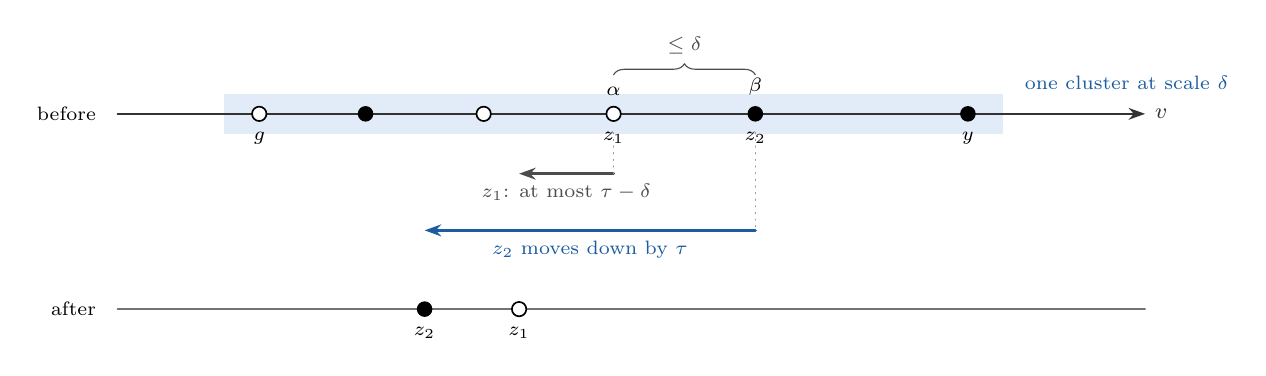
\begin{tikzpicture}[x=30mm,y=8mm]
    \fill[accl] (0.25,-0.32) rectangle (3.55,0.32);
    \draw[axis] (-0.2,0) -- (4.15,0) node[right,lab] {$v$};
    \node[dotO] (g) at (0.4,0) {};
    \node[dotS] at (0.85,0) {};
    \node[dotO] at (1.35,0) {};
    \node[dotO] (z1) at (1.9,0) {};
    \node[dotS] (z2) at (2.5,0) {};
    \node[dotS] (y) at (3.4,0) {};
    \node[slab,below=3pt] at (g) {$g$};
    \node[slab,below=3pt] at (z1) {$z_1$};
    \node[slab,below=3pt] at (z2) {$z_2$};
    \node[slab,below=3pt] at (y) {$y$};
    \node[slab,above=3pt] at (z1) {$\alpha$};
    \node[slab,above=3pt] at (z2) {$\beta$};
    \draw[decorate,decoration={brace,amplitude=4pt},black!70]
      (1.9,0.62) -- (2.5,0.62) node[midway,above=4pt,slab] {$\le\delta$};
    \node[slab,text=acc,anchor=west] at (3.6,0.5) {one cluster at scale $\delta$};
    \draw[->,black!70,line width=1.1pt] (1.9,-0.95) -- (1.5,-0.95)
      node[midway,below,slab] {$z_1$: at most $\tau-\delta$};
    \draw[->,acc,line width=1.1pt] (2.5,-1.85) -- (1.1,-1.85)
      node[midway,below,slab,text=acc] {$z_2$ moves down by $\tau$};
    \draw[black!40,dotted] (1.9,-0.3) -- (1.9,-0.95) (2.5,-0.3) -- (2.5,-1.85);
    \draw[black!55,line width=0.6pt] (-0.2,-3.1) -- (4.15,-3.1);
    \node[dotS] (a2) at (1.1,-3.1) {};
    \node[dotO] (a1) at (1.5,-3.1) {};
    \node[slab,below=3pt] at (a2) {$z_2$};
    \node[slab,below=3pt] at (a1) {$z_1$};
    \node[slab,anchor=east] at (-0.25,-3.1) {after};
    \node[slab,anchor=east] at (-0.25,0) {before};
  \end{tikzpicture}
  \caption{Steps 6 and 7 of the proof of Theorem~\ref{thm:potential}.  Filled
  elements lie in the fully raised blocks $E_{S_0}$, open ones do not.  Inside the cluster joining $g$ and
  $y$, the last open element below $y$ and the next filled element above it are
  consecutive, hence within $\delta$.  The filled one moves by the full $\tau$ and
  the open one by at most $\tau-\delta$, so they cross or meet.}
  \label{fig:cross}
\end{figure}

The pairs of Theorem~\ref{thm:potential} range over all of
$E_{S_0}\times(E\setminus E_{S_0})$.  A fixed minimum base confines them: at every
update some pair with an element in the base crosses, and there are at most $km$
such pairs.  The same base serves for the whole stage, and a pair whose first
element is fully raised stays at or below the second once it gets there, which
bounds a stage independently of $r$.

\begin{theorem}[Stage length]
\label{thm:stagelength}
Let $B$ be a base of $M^{v}$ meeting exactly $r$ blocks, and for $u\in\R^{E}$ let
\[
  R_B(u)=\bigl\{(x,z)\in E\times E:x\ne z,\ x\in B\text{ or }z\in B,\
  \blk(x)\in\Av(M^{u}),\ u_x\le u_z\bigr\}.
\]
\begin{enumerate}
  \item Some $x\in E_{S_0}$ and $z\notin E_{S_0}$ in the same connected component of $M$,
        one of them in $B$, satisfy $v_x>v_z$ and $v'_x\le v'_z$.
  \item If $|S_0|=k-r$ and $\nu(M^{v'})=r$, then $\Av(M^{v'})\ne S_0$.
  \item If $\nu(M^{v'})=r$, then $R_B(v)\subsetneq R_B(v')$.
\end{enumerate}
Consequently stage $r$ ends after at most $\min\bigl(1+(r-1)km,\,1+k(2m-k-1)\bigr)$
updates.
\end{theorem}

\begin{proof}
We use $\delta$ of Step 3 of the proof of Theorem~\ref{thm:potential} and write
$\rho=|S_0|-(k-r)$.

\emph{Step 1: $|B\cap E_{S_0}|=\rho$.}  The $k-r$ blocks that $B$ misses lie in $S_0$, so
$B\cap E_{S_0}$ meets at least $\rho$ blocks, and it is independent in $M^{v}$; by
Lemma~\ref{lem:avoidable}(2),
\[
  \rho\le|B\cap E_{S_0}|\le r_{M^{v}}(E_{S_0})=\rho.
\]
So Step 5 of the proof of Theorem~\ref{thm:potential} applies to $B$: it gives
$g\in B\setminus E_{S_0}$ and $y\in E_{S_0}\setminus B$ in one cluster $\Gamma$ at
scale $\delta$ with $v_g<v_y$, and its last argument gives, for
$f\in E_{S_0}\setminus B$,
\[
  v_c<v_f\qquad\bigl(c\in C(B,f)\setminus E_{S_0}\bigr).
\]

\emph{Step 2: $0<v_x-v_z\le\delta$ for some $x\in E_{S_0}$ and $z\notin E_{S_0}$, one of them in $B$.}  Let
\[
  v_{z_2}=\min\{v_z:z\in\Gamma\cap E_{S_0},\ v_z>v_g\},\qquad
  v_{z_1}=\max\{v_z:z\in\Gamma\setminus E_{S_0},\ v_z<v_{z_2}\},
\]
the sets being nonempty by $y$ and $g$.  Then $v_g\le v_{z_1}<v_{z_2}$, no value
of $\Gamma$ lies in $(v_{z_1},v_{z_2})$, and as in Step 6 of the proof of
Theorem~\ref{thm:potential}, $v_{z_2}-v_{z_1}\le\delta$.  We find $x\in E_{S_0}$ and
$z\notin E_{S_0}$, one of them in $B$, with
\begin{equation}
  0<v_x-v_z\le\delta.
  \label{eq:pair}
\end{equation}
If $z_2\in B$, take $(x,z)=(z_2,z_1)$.  Otherwise $z_2\in\PO_\delta$ lies in
$\cl(C(B,z_2)-z_2)$ but not in $\cl\{f:v_f<v_{z_2}-\delta\}$, so by the minimality
of $B$ some $c\in C(B,z_2)-z_2$ has
\[
  v_{z_2}-\delta\le v_c\le v_{z_2}.
\]
As $c\in B\subseteq\PO_\delta$ lies in the component of $z_2$ and within $\delta$
of it, $c\in\Gamma$, and \eqref{eq:pair} holds, with $x$ and $z$ in the cluster
$\Gamma$ and so in one component, for
\[
  (x,z)=
  \begin{cases}
    (z_2,c),&c\notin E_{S_0},\ \text{where }v_c<v_{z_2}\text{ by Step 1},\\
    (c,z_1),&c\in E_{S_0},\ v_c=v_{z_2},\\
    (z_2,g),&c\in E_{S_0},\ v_c<v_{z_2},
  \end{cases}
\]
in the last case because $v_c\le v_g$ by the choice of $z_2$, so that
$0<v_{z_2}-v_g\le v_{z_2}-v_c\le\delta$.

\emph{Step 3: item 1.}  By Steps 2 and 3 of the proof of
Theorem~\ref{thm:potential} and \eqref{eq:pair},
\[
  v'_x-v'_z\le(v_x-\tau)-\bigl(v_z-(\tau-\delta)\bigr)=(v_x-v_z)-\delta\le0.
\]

\emph{Step 4: item 2.}  Let $\rho=0$, and suppose $\nu(M^{v'})=r$ and
$\Av(M^{v'})=S_0$.  By \eqref{eq:jump}, $r_{N(\delta)}(E_{S_0})>0$, so some
$y\in E_{S_0}$ lies in a base of $N(\delta)$, hence in $\PO_\delta$.  By
Lemma~\ref{lem:avoidable}(2) for $M^{v'}$, $r_{M^{v'}}(E_{S_0})=\rho=0$, so a
minimum base $B'$ of $v'$ misses $E_{S_0}$, and the last argument of Step 1, at
$v'$ and $B'$, gives $v'_f<v'_y$ for $f\in C(B',y)-y$.  By Step 3 of the proof of
Theorem~\ref{thm:potential},
\[
  v_f\le v'_f+(\tau-\delta)<v'_y+(\tau-\delta)=v_y-\delta\qquad\bigl(f\in C(B',y)-y\bigr),
\]
so $y\in\cl\bigl(C(B',y)-y\bigr)\subseteq\cl\{f:v_f<v_y-\delta\}$, against
$y\in\PO_\delta$.

\emph{Step 5: at most $1+(r-1)km$ updates.}  Call a maximal run of updates of stage $r$
that start
from states with the same $S_0$ a \emph{phase}.  By Theorem~\ref{thm:potential}(1)
and Step 8 of its proof, $S_0$ grows strictly from one phase to the next and
$0\le\rho\le r-1$, so the phases have distinct values of $\rho$, and by item 2 the
phase with $\rho=0$, if any, has one update.  In a phase with $\rho\ge1$ fix a
base $B$ of $M^{v}$ meeting exactly $r$ blocks at its first state; by Theorem~\ref{thm:validity}(2) it is a base of $M^{v}$
meeting $r$ blocks at every state of the phase.  Let
\[
  \Phi(v)=\bigl|\{(x,z):x\in E_{S_0},\ z\notin E_{S_0},\ x\in B\text{ or }z\in B,\
  v_x>v_z\}\bigr|,
\]
formed with the $S_0$ of the phase.  At an update $v\to v'$ of the phase, by Step 2
of the proof of Theorem~\ref{thm:potential} no pair with $v_x\le v_z$ has
$v'_x>v'_z$, and by item 1 some pair counted by $\Phi(v)$ has $v'_x\le v'_z$, so
$\Phi(v')\le\Phi(v)-1$, while
\[
  \Phi(v)\le|B\cap E_{S_0}|\,|E\setminus E_{S_0}|+|E_{S_0}|\,|B\setminus E_{S_0}|\le|B|\,m=km.
\]
So a phase with $\rho\ge1$ has at most $km$ updates, and stage $r$ has at most
$1+(r-1)km$.

\emph{Step 6: item 3.}  Let $\nu(M^{v'})=r$ and $(x,z)\in R_B(v)$.  By
Theorem~\ref{thm:potential}(1), $\blk(x)\in S_0\subseteq\Av(M^{v'})$, and by Step 2
of its proof, $a_{\blk(x)}=\tau\ge a_{\blk(z)}$, so
\[
  v'_x-v'_z=(v_x-\tau)-\bigl(v_z-a_{\blk(z)}\bigr)\le v_x-v_z\le0,
\]
and $(x,z)\in R_B(v')$.  The pair $(x,z)$ of item 1 has $x\ne z$, as $\blk(x)\in S_0$
and $\blk(z)\notin S_0$; it lies outside $R_B(v)$, as $v_x>v_z$, and in $R_B(v')$,
as $\blk(x)\in S_0\subseteq\Av(M^{v'})$ and $v'_x\le v'_z$.

\emph{Step 7: at most $1+k(2m-k-1)$ updates.}  Let stage $r$ consist of the updates
$v^{j}\to v^{j+1}$, $j<n$, so that $\nu(M^{v^{j}})=r$ for $j<n$, and let $B$ be a base
of $M^{v^{0}}$ meeting exactly $r$ blocks.  By Theorem~\ref{thm:validity}(2) and
induction on $j$, $B$ is a base of $M^{v^{j}}$ meeting exactly $r$ blocks for every
$j<n$, so item 3 applies with this $B$ at every update $v^{j}\to v^{j+1}$ with
$j<n-1$.  As $R_B(v^{n-1})$ consists of pairs $(x,z)$ with $x\ne z$ and $x$ or $z$
in $B$, and $|B|=k$,
\[
  n-1\le\bigl|R_B(v^{n-1})\bigr|-\bigl|R_B(v^{0})\bigr|\le k(m-1)+(m-k)k=k(2m-k-1).
\]
With Step 5, stage $r$ has at most $\min\bigl(1+(r-1)km,\,1+k(2m-k-1)\bigr)$ updates.
\end{proof}

When the components are as small as possible, the pair of item 1 ends the phase at
once.

\begin{corollary}
\label{cor:rankone}
If every connected component of $M$ has rank at most one, every update of stage $r$
changes $S_0$ or ends the stage, and stage $r$ ends after at most $r$ updates.
\end{corollary}

\begin{proof}
\emph{Step 1: $\{x,z\}$ is a circuit.}  Let $B$, $x$ and $z$ be as in
Theorem~\ref{thm:stagelength}(1).  Since $x\in E_{S_0}$ and $z\notin E_{S_0}$, $x\ne z$, and
as their component has rank one, $\{x,z\}$ is a circuit.

\emph{Step 2: $z\in B$ and $x\notin B$.}  If $x\in B$, then $z\notin B$ and $C(B,z)=\{x,z\}$, and
Lemma~\ref{lem:minbases}(1) would give
\[
  v_x\le v_z<v_x.
\]
So $z\in B$, $x\notin B$ and $C(B,x)=\{x,z\}$.

\emph{Step 3: $\nu(M^{v'})>r$ or $\Av(M^{v'})\supsetneq S_0$.}  By Theorem~\ref{thm:validity}(2), $B$ is a minimum base
of $v'$, so by Lemma~\ref{lem:minbases}(1) and Theorem~\ref{thm:stagelength}(1),
\[
  v'_z\le v'_x\le v'_z,
\]
and by Lemma~\ref{lem:minbases}(3) $B-z+x$ is a minimum base of $v'$ with
\[
  |(B-z+x)\cap E_{S_0}|=|B\cap E_{S_0}|+1=\rho+1,
\]
by Step 1 of the proof of Theorem~\ref{thm:stagelength}.  If $\nu(M^{v'})=r$ and
$\Av(M^{v'})=S_0$, then Lemma~\ref{lem:avoidable}(2) for $M^{v'}$ gives
\[
  \rho+1=|(B-z+x)\cap E_{S_0}|\le r_{M^{v'}}(E_{S_0})=|S_0|-(k-r)=\rho,
\]
a contradiction.  So $\nu(M^{v'})>r$ or $\Av(M^{v'})\supsetneq S_0$ by
Theorem~\ref{thm:potential}(1).

\emph{Step 4: at most $r$ updates.}  By Step 8 of the proof of Theorem~\ref{thm:potential},
$k-r\le|S_0|\le k-1$ within the stage, and by Step 3 every update of the stage
that does not end it increases $|S_0|$.  So the stage has at most
$(k-1)-(k-r)+1=r$ updates.
\end{proof}

\subsection{The circuit}
\label{sec:circuit}

The tests behind an update are questions of unweighted matroid
intersection, and the augmenting path algorithm answers them without branching
on weights.

\begin{lemma}
\label{lem:augment}
Let $N_x$ be a matroid on $E$ for every vector $x$ of input bits, and for each
$y\in E$ let a Boolean circuit of size $q$ decide, from $x$ and the indicator
vector of a set $J$ with $y\in J$ and $J-y$ independent in $N_x$, whether $J$ is
independent in $N_x$.  For $j\ge0$, a Boolean circuit with
$j(m^{2}q+8m^{3}+12m^{2}+12m+4)$ gates computes from $x$ the indicator vector of
a rainbow independent set of $N_x$ with at least $\min(j,\nu(N_x))$ elements, and
with $\nu(N_x)$ elements for $j=k$.  For $r_0\ge0$, a Boolean circuit of size at
most
\[
  (r_0+2)(m+1)^{2}\bigl(q+10(m+1)\bigr)+3k(m+1)+5\lceil\log_2(r_0+1)\rceil
\]
computes from $x$ the $k$ bits
$\mathbf 1[\nu(N_x)\le r_0]\wedge\mathbf 1[b\in\Av(N_x)]$.
\end{lemma}

\begin{proof}
\emph{Step 1: a round of $m^{2}q+8m^{3}+12m^{2}+12m+4$ gates enlarges $I$ unless $|I|=\nu(N_x)$.}  From the indicator vector of a rainbow independent set
$I$, a round builds the exchange graph $D_I$ of the proof of
Lemma~\ref{lem:avoidable}: the circuit of $y$ tests $I-x'+y$ for the arcs
$y\to x'$ and $I+y$ for the sinks, and the sources and the arcs inside blocks are
read from $I$.  An answer is used only when $y\notin I$, and for an arc only when
$x'\in I$; the bits of $I$ mask the others.  The used sets contain $y$, and
removing $y$ leaves $I-x'$ or $I$, which are independent, so the circuits answer
them.  With a breadth-first search from the sources, the sink of least index in
the first layer containing a sink, the predecessors of least index and the
exchange along this shortest path, a round costs
\[
  \underbrace{m(m-1)q}_{\text{arcs}}+\underbrace{mq}_{\text{sinks}}
  +\underbrace{8m^{3}+12m^{2}+12m+4}_{\text{search and exchange}}
  =m^{2}q+8m^{3}+12m^{2}+12m+4.
\]
By the exchange lemma for shortest paths~\cite{schrijver03} the new set is
rainbow, independent and has $|I|+1$ elements, and if no sink is reachable, $I$
is maximum and is kept~\cite{lawler75,schrijver03}.

\emph{Step 2: $\min(j,\nu(N_x))\le|I|\le\nu(N_x)$ after $j$ rounds.}  From $I=\varnothing$, $|I|$ grows by one per round
until $|I|=\nu(N_x)\le k$, so $j$ rounds give
\[
  \min\bigl(j,\nu(N_x)\bigr)\le|I|\le\nu(N_x),
\]
and $k$ rounds give $|I|=\nu(N_x)$.

\emph{Step 3: the bits $\mathbf 1[\nu(N_x)\le r_0]\wedge\mathbf 1[b\in\Av(N_x)]$.}  Run $j=r_0+1$ rounds.  If $\nu(N_x)\le r_0$, then
$|I|=\nu(N_x)$ by Step 2, and one more exchange graph ($m(m-1)$ tests) and its
reachable set $Z$ ($2m^{3}$ gates) give, by Steps 2 to 6 of the proof of
Lemma~\ref{lem:avoidable},
\[
  \Av(N_x)=\{b:b\text{ missed by }I\}\cup\blk(I\cap Z).
\]
If $\nu(N_x)>r_0$, then $|I|\ge r_0+1$ by Step 2.  In both cases
\[
  \mathbf 1\bigl[|I|\le r_0\bigr]\wedge\mathbf 1\bigl[b\in\{b:b\text{ missed by }I\}\cup\blk(I\cap Z)\bigr]
  =\mathbf 1\bigl[\nu(N_x)\le r_0\bigr]\wedge\mathbf 1\bigl[b\in\Av(N_x)\bigr].
\]
A population count of $I$, a comparison with $r_0$ and $k$ conjunctions complete
the outputs, within
$(r_0+2)(m+1)^{2}(q+10(m+1))+3k(m+1)+5\lceil\log_2(r_0+1)\rceil$ gates.
\end{proof}

\begin{lemma}
\label{lem:observer}
Let $M$ have a Boolean rank circuit of size $s$, and fix
$r_0\in\{1,\ldots,k-1\}$.  For
$v\in\R^{E}$ let $\mathcal Q(v)$ be the vector of the $m+2m^{2}$ values $t_x$,
$T_{xy}$ and $\omega_{xy}$ of Lemma~\ref{lem:events}, with $T_{xy}=\omega_{xy}=0$ for
$x,y$ not joined.  A Boolean circuit of size $O(r_0m^{2}(s+m))$ reads $m+2m^{2}$
bits and outputs $k$ bits $F_b$, $b\in[k]$, such that on input
$\mathbf 1[\mathcal Q(v)\le t]$
\[
  F_b=\mathbf 1\bigl[\nu(N(t))\le r_0\bigr]\wedge\mathbf 1\bigl[b\in\Av(N(t))\bigr]
\]
for every $v\in\R^{E}$ and $t\ge0$, where $N(t)$ is the family of
Definition~\ref{def:posl} for $v$.
\end{lemma}

\begin{proof}
Fix $v$ and $t\ge0$, and write $\PO=\PO_t$, $u=u_t$ and $N_t=N(t)$.

\emph{Step 1: $\PO$, the clusters and their order with $2m^{2}$ gates.}  The loops and the connected components of $M$ are
fixed, and by Lemma~\ref{lem:events}, at the bits $\mathbf 1[\mathcal Q(v)\le t]$,
\[
  x\in\PO\iff x\text{ is a non-loop and }t_x\le t,
\]
two distinct elements lie in one cluster if and only if they are joined and
$T_{xy}\le t$, and for $x,y$ in one component
\[
  u(x)<u(y)\iff x,y\text{ joined},\ t_x\le t\ \text{and not}\ \omega_{xy}\le t.
\]
So the bits of $\PO$ and of the clusters cost no gate, and the order bits cost
$2m^{2}$ gates.

\emph{Step 2: the independence test of $N_t$ with $q=s+O(m)$ gates.}  For $y\in\PO$ let $\mathrm{Lev}(y)$ be the cluster
of $y$ and $\mathrm{Below}(y)$ the set of elements of its component with smaller
$u$; both depend only on the cluster.  By \eqref{eq:rank-mu} within components,
\[
  r_{N_t}(A)=\sum_{x}\kappa_x(A),\qquad
  \kappa_x(A)=r_M\bigl(\mathrm{Below}(x)\cup(A\cap\mathrm{Lev}(x))\bigr)-r_M\bigl(\mathrm{Below}(x)\bigr),
\]
the sum over one element $x$ of each cluster; the set $E\setminus\PO=\{u=m+1\}$
contributes $0$, as $\PO\supseteq\PO_0$ spans $E$.  Each term satisfies
$\kappa_x(A)\le|A\cap\mathrm{Lev}(x)|$, and the clusters partition $\PO$, so
\[
  r_{N_t}(A)\le\sum_x|A\cap\mathrm{Lev}(x)|=|A\cap\PO|\le|A|,
\]
and $A$ is independent in $N_t$ if and only if $A\subseteq\PO$ and
$\kappa_x(A)=|A\cap\mathrm{Lev}(x)|$ for every $x$.  Let $y\in A$ with $A-y$
independent, so that $A-y\subseteq\PO$ and, for $x$ outside the cluster of $y$,
\[
  \kappa_x(A)=\kappa_x(A-y)=|(A-y)\cap\mathrm{Lev}(x)|=|A\cap\mathrm{Lev}(x)|.
\]
Hence
\[
  A\text{ independent in }N_t\iff y\in\PO\ \text{and}\
  r_M\bigl(\mathrm{Below}(y)\cup(A\cap\mathrm{Lev}(y))\bigr)
  =r_M\bigl(\mathrm{Below}(y)\bigr)+|A\cap\mathrm{Lev}(y)|.
\]
The ranks $r_M(\mathrm{Below}(y))$ cost $ms$ gates once, and then this test costs
$q=s+O(m)$ gates: the sets $A\cap\mathrm{Lev}(y)$ and
$\mathrm{Below}(y)\cup(A\cap\mathrm{Lev}(y))$, one rank evaluation, a subtraction,
a population count, a comparison and a conjunction with $\mathbf 1[y\in\PO]$.

\emph{Step 3: the bits $F_b$ with $O(r_0m^{2}(s+m))$ gates.}  Lemma~\ref{lem:augment}, with the input bits and
the data of Steps 1 and 2 as its input, the matroids $N_t$ and the tests of Step 2,
gives the bits $F_b$ from $r_0+1$ rounds with
\[
  (r_0+2)(m+1)^{2}\bigl(q+10(m+1)\bigr)+3k(m+1)+5\lceil\log_2(r_0+1)\rceil
  =O\bigl(r_0m^{2}(s+m)\bigr)
\]
gates, as $k\le m$, and Steps 1 and 2 cost $ms+2m^{2}$ gates besides the tests.
\end{proof}

\begin{lemma}
\label{lem:oneupdate}
Let $M$ have a Boolean rank circuit of size $s$.  For each stage $r$, a
$(\max,+,-)$-circuit of size $O(rm^{3}(s+m))$ maps
$(w,p)$ to $p+a$, with $a$ the PO-SL update at $v=w-p_{\blk}$, at every state
with $\nu_0\ge r$.
\end{lemma}

\begin{proof}
\emph{Step 1: $v$ with $m$ gates.}  One subtraction per element gives $v=w-p_{\blk}$.

\emph{Step 2: $\Lambda$ and $\mathcal Q(v)$ with $O(m^{2}s+m^{3})$ gates.}  For a non-loop $x$, the vector $D^{x}$ costs $2m$
gates and the Boolean circuit of $\phi_x(S)=\mathbf 1[r_M(E\setminus S+x)=r_M(E\setminus S)]$,
with $m$ negations, two rank evaluations and a comparison, has $2s+O(m)$ gates, so
Theorem~\ref{thm:compiler} gives $t_x$ with $O(ms+m^{2})$ gates.  Let $\mathcal J$ be the
set of joined pairs, so that $W\in\R^{\mathcal J}$.  The Floyd--Warshall algorithm
$\mathrm{FW}$ over $(\min,\max)$ starts from $W$ and replaces $T_{xy}$ by
$\min(T_{xy},\max(T_{xz},T_{zy}))$ for the pivots $z$ in turn, and Warshall's
algorithm~\cite{warshall62} does the same on bits with $\vee$ and $\wedge$.  As
\[
  \mathbf 1\bigl[\min(T_{xy},\max(T_{xz},T_{zy}))\le t\bigr]
  =\mathbf 1[T_{xy}\le t]\vee\bigl(\mathbf 1[T_{xz}\le t]\wedge\mathbf 1[T_{zy}\le t]\bigr),
\]
every pivot commutes with the threshold map, so for every $t\ge0$
\[
  \begin{tikzcd}[column sep=4.5em,row sep=2.2em]
    \R^{\mathcal J}\arrow[r,"\mathrm{FW}"]\arrow[d,"{\mathbf 1[\,\cdot\,\le t]}"'] &
    \R^{\mathcal J}\arrow[d,"{\mathbf 1[\,\cdot\,\le t]}"]\\
    \{0,1\}^{\mathcal J}\arrow[r,"\text{Warshall}"'] & \{0,1\}^{\mathcal J}
  \end{tikzcd}
\]
commutes, and $\mathrm{FW}(W)$ is the matrix of the least values $T_{xy}$ of
Lemma~\ref{lem:events}(2).  With the
values $\sigma_x$ and $\omega_{xy}$, the levels $\Lambda$ and the values
$\mathcal Q(v)$ cost
\[
  \underbrace{O(m^{2}s+m^{3})}_{t_x}+\underbrace{5m^{2}}_{W}+\underbrace{4m^{3}}_{T}
  +\underbrace{3m^{2}}_{\sigma}+\underbrace{6m^{2}}_{\omega}=O(m^{2}s+m^{3})
\]
gates.

\emph{Step 3: $a_b=\sum_{i<2m}\Delta_i\,F_b(\mathbf 1[\mathcal Q(v)\le d_i])$.}  Let $F_b$ be the bits of
Lemma~\ref{lem:observer} with $r_0=r$, and for a matroid $N$ on $E$ let
$\chi_b(N)=\mathbf 1[\nu(N)\le r]\wedge\mathbf 1[b\in\Av(N)]$.  By
Lemma~\ref{lem:observer}, for every $v\in\R^{E}$
\[
  \begin{tikzcd}[column sep=5.4em,row sep=2.4em]
    {[0,\infty)}\arrow[r,"{t\,\mapsto\,\mathbf 1[\mathcal Q(v)\le t]}"]
      \arrow[d,"{t\,\mapsto\,N(t)}"'] &
    \{0,1\}^{m+2m^{2}}\arrow[d,"F_b"]\\
    \{\text{matroids on }E\}\arrow[r,"\chi_b"'] & \{0,1\}
  \end{tikzcd}
\]
commutes.  Let $0=d_0\le\cdots\le d_{2m}$ be the entries of
$\Lambda$ in increasing order with a zero prepended.  Every entry of $\mathcal Q(v)$
lies in $\Lambda\cup\{0\}$ by Lemma~\ref{lem:events}, so the bits
$\mathbf 1[\mathcal Q(v)\le t]$ are constant on each $[d_i,d_{i+1})$, and for
$t\ge d_{2m}$ they are all $1$, as at $t'=\max(d_{2m},\max v-\min v)$, where
$N(t')=M$ by Step 4 of the proof of Proposition~\ref{prop:posl} and $\nu(M)=k>r$.
So for $t\ge d_{2m}$, by the square,
\[
  F_b\bigl(\mathbf 1[\mathcal Q(v)\le t]\bigr)=F_b\bigl(\mathbf 1[\mathcal Q(v)\le t']\bigr)
  =\chi_b(M)=0.
\]
If $\nu_0=r$, then by \eqref{eq:update-integral} and the square,
\[
  \begin{aligned}
  a_b&=\int_0^{\infty}\chi_b\bigl(N(t)\bigr)\,dt
  =\int_0^{\infty}F_b\bigl(\mathbf 1[\mathcal Q(v)\le t]\bigr)\,dt\\
  &=\sum_{i=0}^{2m-1}\Delta_i\,F_b\bigl(\mathbf 1[\mathcal Q(v)\le d_i]\bigr),
  \end{aligned}
\]
and if $\nu_0>r$, then $\nu(N(t))\ge\nu_0>r$ for all $t$ and both sides are
$0=a_b$.

\emph{Step 4: $a$ with $O(rm^{3}(s+m))$ gates.}  Corollary~\ref{cor:levels} with the $2m$
levels $\Lambda$, the $m+2m^{2}$ values $\mathcal Q(v)$ as $Y$ and the $k$ outputs
$F_b$, applied to the circuit of Lemma~\ref{lem:observer}, gives $a$ with
\[
  6m^{2}+2m\Bigl(1+4(m+2m^{2})+3\cdot O\bigl(rm^{2}(s+m)\bigr)+k\Bigr)
  =O\bigl(rm^{3}(s+m)\bigr)
\]
gates.

\emph{Step 5: $p+a$ with $k$ gates.}  One addition per block gives $p+a$.
\end{proof}

\begin{proof}[Proof of Theorem~\ref{thm:C}]
\emph{Step 1: $\ell_r$ updates of stage $r$ for $r=1,\ldots,k-1$.}  Start from $p=0$, where $\nu_0\ge1$ since a minimum
base of $w$ meets some block.  For $r=1,\ldots,k-1$ apply the circuit of
Lemma~\ref{lem:oneupdate} for stage $r$, which is the identity at $\nu_0>r$ as
$a=0$ there, exactly $\ell_r$ times, where
\[
  \ell_r=\min\bigl(r(\lfloor m^{2}/4\rfloor+1),\,1+(r-1)km,\,1+k(2m-k-1)\bigr).
\]

\emph{Step 2: $\nu_0=k$ after stage $k-1$.}  By induction on $r$, $\nu_0\ge r$ at the start of
stage $r$.  As $\nu_0$ never decreases (Theorem~\ref{thm:validity}(2)) and
Theorems~\ref{thm:potential} and~\ref{thm:stagelength} bound the number of
updates at $\nu_0=r$ by $\ell_r$, we have $\nu_0\ge r+1$ after stage $r$, and
$\nu_0=k$ after stage $k-1$.

\emph{Step 3: the output $\Psi(p)=\Opt(w)$.}  By Lemma~\ref{lem:duality} and Theorem~\ref{thm:A},
at $O(ms+m^{2})$ further gates the circuit outputs
\[
  \Psi(p)=\sum_{b=1}^{k}p_b+\beta_M(v)=\sum_{b=1}^{k}p_b-h_M(-v)=\Opt(w).
\]

\emph{Step 4: the size is $O(k^{3}m^{4}(s+m))$, and the family is uniform.}  The number of updates is at most
\[
  \sum_{r=1}^{k-1}\ell_r\le(k-1)\bigl(1+k(2m-k-1)\bigr)\le(k-1)(1+2km)
  =2k^{2}m-(2km-k+1)\le2k^{2}m.
\]
An update of stage $r$ has $O(rm^{3}(s+m))$ gates by Lemma~\ref{lem:oneupdate},
and $\ell_r\le1+k(2m-k-1)\le2km$, so
\[
  \sum_{r=1}^{k-1}r\,\ell_r\le2km\sum_{r=1}^{k-1}r=k^{2}(k-1)m\le k^{3}m.
\]
So the size is $O(k^{3}m^{4}(s+m))$.  If every connected component of $M$ has
rank at most one, Corollary~\ref{cor:rankone} allows $\ell_r=r$ in Step 1, and then the size is $O(k^{3}m^{3}(s+m))$, as
\[
  \sum_{r=1}^{k-1}r\,\ell_r=\sum_{r=1}^{k-1}r^{2}\le k^{3}.
\]  The circuit depends only on $M$, the
blocks and the rank circuit.  Besides them it uses the rank $k=r_M(E)$ and the
connected components of $M$, which a polynomial-time algorithm obtains from the
rank circuit: $k$ by one evaluation, a base $B_0$ by the greedy algorithm, each
fundamental circuit $C(B_0,e)$ by $k$ evaluations, and the components as the
classes of the transitive closure of ``$e$ and $f$ lie in a common fundamental
circuit of $B_0$''~\cite{oxley11}.  So the family is uniform.
\end{proof}

\section{Two matroids}
\label{sec:two}

Common bases of two matroids are rainbow bases of a third one on twice as many
elements, with one block for the two copies of each element, so
Theorem~\ref{thm:C} applies to weighted matroid intersection without change.

\begin{lemma}
\label{lem:doubling}
Let $M_1,M_2$ be matroids of rank $\rho$ on $E$.  On $E\times\{1,2\}$ let
$N=M_1\oplus M_2^{*}$, with blocks $\{(e,1),(e,2)\}$ and weight $w_e$ on $(e,1)$,
$0$ on $(e,2)$.  For $X\subseteq E$, the set $X\times\{1\}\cup(E\setminus X)\times\{2\}$,
which meets every block once, is a base of $N$ if and only if $X$ is a common base
of $M_1$ and $M_2$, and its weight is $w(X)$.  Every rainbow base of $N$ has this
form.
\end{lemma}

\begin{proof}
\emph{Step 1: $X\times\{1\}\cup(E\setminus X)\times\{2\}\in\Bases(N)\iff X\in\Bases(M_1)\cap\Bases(M_2)$.}  Since the bases of $M_2^{*}$ are the complements of
the bases of $M_2$,
\[
  X\times\{1\}\cup(E\setminus X)\times\{2\}\in\Bases(N)
  \iff X\in\Bases(M_1),\ E\setminus X\in\Bases(M_2^{*})
  \iff X\in\Bases(M_1)\cap\Bases(M_2),
\]
and only the first copies carry weight, so the weight is $w(X)$.

\emph{Step 2: every rainbow base of $N$ has this form.}  $N$ has rank $\rho+(m-\rho)=m$, so a rainbow
base meets each of the $m$ blocks once, and it is the set of Step 1 for the set
$X$ of elements whose first copy it contains.
\end{proof}

\begin{figure}[t]
  \centering
  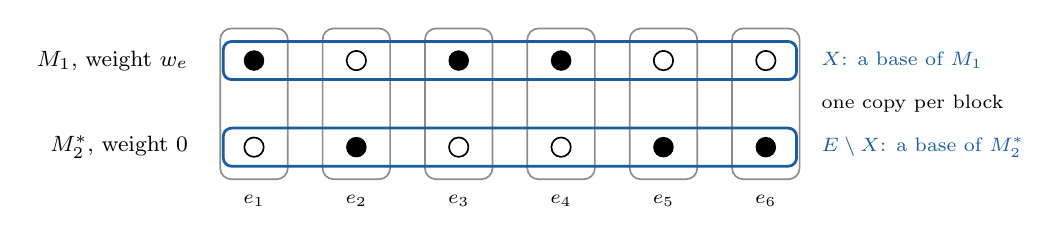
\begin{tikzpicture}[x=13mm,y=11mm]
    \foreach \e in {1,...,6} {
      \draw[black!45,rounded corners=4pt,line width=0.6pt]
        (\e-0.33,-0.37) rectangle (\e+0.33,1.37);
      \node[slab] at (\e,-0.62) {$e_{\e}$};}
    \foreach \e in {1,3,4} {
      \node[dotS,minimum size=7pt] at (\e,1) {};
      \node[dotO,minimum size=7pt] at (\e,0) {};}
    \foreach \e in {2,5,6} {
      \node[dotO,minimum size=7pt] at (\e,1) {};
      \node[dotS,minimum size=7pt] at (\e,0) {};}
    \node[lab,anchor=east] at (0.45,1) {$M_1$, weight $w_e$};
    \node[lab,anchor=east] at (0.45,0) {$M_2^{*}$, weight $0$};
    \draw[acc,line width=1pt,rounded corners=3pt] (0.7,0.78) rectangle (6.3,1.22);
    \draw[acc,line width=1pt,rounded corners=3pt] (0.7,-0.22) rectangle (6.3,0.22);
    \node[slab,text=acc,anchor=west] at (6.45,1) {$X$: a base of $M_1$};
    \node[slab,text=acc,anchor=west] at (6.45,0) {$E\setminus X$: a base of $M_2^{*}$};
    \node[slab,anchor=west] at (6.45,0.5) {one copy per block};
  \end{tikzpicture}
  \caption{Lemma~\ref{lem:doubling}.  Each block is a column holding the two
  copies of an element; a rainbow base picks one copy per column (filled), the
  first copies forming $X$ and the second copies $E\setminus X$.}
  \label{fig:double}
\end{figure}

\begin{proof}[Proof of Theorem~\ref{thm:D}]
\emph{Step 1: $\Opt(w)$ for $N$ is the minimum weight of a common base.}  If $M_1$ and $M_2$ have a common base, both have
rank $\rho$, and $N$ of Lemma~\ref{lem:doubling} has rank $m$ on $2m$ elements
with $m$ blocks, its rainbow bases corresponding to the common bases with equal
weights (Figure~\ref{fig:double}).

\emph{Step 2: a rank circuit of $N$ with $s_1+s_2+O(m)$ gates.}  With $r_i$ the rank function of $M_i$, for
$X_1,X_2\subseteq E$,
\[
  r_N\bigl(X_1\times\{1\}\cup X_2\times\{2\}\bigr)=r_1(X_1)+r_2^{*}(X_2)=r_1(X_1)+|X_2|+r_2(E\setminus X_2)-r_2(E),
\]
computed from the two rank circuits, the second on the negated indicator vector
of $X_2$, a population count, two additions and the subtraction of the constant
$r_2(E)$ on $O(\log m)$ bits, at $s_1+s_2+O(m)$ gates.

\emph{Step 3: the minimum weight of a common base with $O(m^{7}(s_1+s_2+m))$ gates.}  Theorem~\ref{thm:C} with $2m$ elements, $k=m$
blocks and the weights of Lemma~\ref{lem:doubling} gives the minimum weight of a
common base with
\[
  O\bigl(m^{3}(2m)^{4}(s_1+s_2+m)\bigr)=O\bigl(m^{7}(s_1+s_2+m)\bigr)
\]
gates.  The rank circuit of Step 2 is produced from the two given ones in
polynomial time, with $r_2(E)$ found by one evaluation, so the family is uniform
by Theorem~\ref{thm:C}.

\emph{Step 4: $X\cup Y\in\Bases(M_1')\cap\Bases(M_2')\iff X\in\mathcal I,\ |X|+|Y|=m$.}  Let $\mathcal I$ be the family of common
independent sets of $M_1$ and $M_2$, let $Z$ be a set of $m$ new elements, and
for $i=1,2$ let $M_i'$ be the matroid on $E\cup Z$ whose independent sets are the
sets $X\cup Y$ with $X$ independent in $M_i$, $Y\subseteq Z$ and
$|X|+|Y|\le m$: the truncation at $m$ of the direct sum of $M_i$ and the free
matroid on $Z$.  It has rank $m$ and the rank function
\[
  r_i'(S)=\min\bigl(r_i(S\cap E)+|S\cap Z|,\,m\bigr),
\]
which the rank circuit of $M_i$, a population count, an addition and a
comparison with $m$ compute at $s_i+O(m)$ gates.  Its bases are its independent
sets of size $m$, so for $X\subseteq E$ and $Y\subseteq Z$
\[
  X\cup Y\in\Bases(M_1')\cap\Bases(M_2')\iff X\in\mathcal I,\ |X|+|Y|=m,
\]
and $Z$ is a common base of $M_1'$ and $M_2'$.

\emph{Step 5: the maximum weight of a common independent set with $O(m^{7}(s_1+s_2+m))$ gates.}  Let $w'$ be $-w$ on $E$ and $0$ on $Z$, so
that $w'(X\cup Y)=-w(X)$.  Every $X\in\mathcal I$ has $|X|\le m=|Z|$, so by Step 4
\[
  \max_{X\in\mathcal I}w(X)=-\min_{X\in\mathcal I}\bigl(-w(X)\bigr)
  =-\min_{B\in\Bases(M_1')\cap\Bases(M_2')}w'(B).
\]
Step 3 for $M_1'$ and $M_2'$ on $2m$ elements, $m$ negations for $-w$ and one
for the output give this value with $O(m^{7}(s_1+s_2+m))$ gates, and the rank
circuits of $M_1'$ and $M_2'$ are produced in polynomial time as well.
\end{proof}

\paragraph{Transversal matroids and gammoids.}
The circuit of Lemma~\ref{lem:augment} computes the largest size of a rainbow
independent set, that is, it solves unweighted matroid intersection with a
partition matroid.  Transversal matroids have rank functions of this kind, and
gammoids are restrictions of their duals, so Theorem~\ref{thm:A} applies to
both.

\begin{corollary}
\label{cor:transversal}
The following matroids $M$ on $m$ elements have Boolean rank circuits and $(\max,+,-)$-circuits for $h_M$ of polynomial size.
\begin{enumerate}
  \item Let $A_1,\ldots,A_n\subseteq E$, $|E|=m$, and $p=|A_1|+\cdots+|A_n|\le mn$.
        The partial transversals, the sets $X\subseteq E$ with an injective map
        $\phi:X\to[n]$ such that $x\in A_{\phi(x)}$ for every $x\in X$, are the
        independent sets of a matroid $M$, the transversal matroid.  It has a
        Boolean rank circuit of size at most $36(n+1)(p+1)^{2}(m+p+1)$, and $h_M$
        has a $(\max,+,-)$-circuit of size at most
        $120(m+1)(n+1)(p+1)^{2}(m+p+1)\le120(m+1)^{4}(n+1)^{4}$.
  \item Let $D$ be a directed graph on a set $V$ of $v$ vertices whose $a$ arcs are
        ordered pairs of vertices, and let $S,E\subseteq V$ with $|E|=m$.  A set
        $X\subseteq E$ is \emph{linked} from $S$ if there are directed paths, one
        from a vertex of $S$ to each $x\in X$, no two of which share a vertex; a
        vertex of $S\cap X$ is linked by the path without arcs.  The sets linked
        from $S$ are the independent sets of a matroid $M$, the gammoid.  It has a
        Boolean rank circuit of size at most $48(v+1)(v+a+1)^{2}(2v+a+1)$, and
        $h_M$ has a $(\max,+,-)$-circuit of size at most
        $160(m+1)(v+1)(v+a+1)^{2}(2v+a+1)\le160(v+1)^{8}$.
\end{enumerate}
\end{corollary}

\begin{proof}
\emph{Step 1: $\max\{|X|:X\subseteq U\text{ a partial transversal}\}=\nu(N_U)$.}  For $U\subseteq E$ let
$N_U$ be the matroid on the $p$ incidences $(e,i)$, $e\in A_i$, in which a set is
independent when it contains at most one incidence of each element and only
incidences of elements of $U$, with the blocks $R_i=\{(e,i):e\in A_i\}$.  Rainbow
independent sets of $N_U$ are matchings of elements of $U$ into distinct sets,
so
\[
  \max\{|X|:X\subseteq U\text{ a partial transversal}\}=\nu(N_U).
\]

\emph{Step 2: the partial transversals form a matroid with $r(U)=\nu(N_U)$.}  Subsets of partial transversals are partial
transversals.  Let $X,Y$ be partial transversals such that $X+y$ is none for
$y\in Y\setminus X$, let $Q=\Av(N_X)$ and $E_Q$ the incidences in the blocks of
$Q$, and put $A_Q=\bigcup_{i\in Q}A_i$.  An element $y\in Y\cap A_Q$ lies in $X$,
since a matching of $X$ missing the set $A_i\ni y$, $i\in Q$, would extend to
$X+y$.  Hence
\[
  r_{N_Y}(E_Q)=|Y\cap A_Q|\le|X\cap A_Q|=r_{N_X}(E_Q),
\]
and Lemma~\ref{lem:avoidable}(2) for $N_X$ and~(1) for $N_Y$, with
$\nu(N_X)=|X|$ and $\nu(N_Y)=|Y|$ by Step 1, give
\[
  n-|X|=|Q|-r_{N_X}(E_Q)\le|Q|-r_{N_Y}(E_Q)\le n-|Y|.
\]
So the partial transversals form a matroid, as Edmonds and Fulkerson
showed~\cite{oxley11}, with rank function $r(U)=\nu(N_U)$ by Step 1.

\emph{Step 3: the bounds of item 1.}  The set $J$ is independent in
$N_U$ if and only if
\[
  |J|=r_{N_U}(J)=\bigl|\{e\in U:(e,i)\in J\text{ for some }i\}\bigr|,
\]
a test of at most $28p+23m+1$ gates with the bits of $U$ as extra inputs: one
disjunction per incidence, one conjunction per element and two population
counts.  Lemma~\ref{lem:augment} on the $p$ incidences and $n$ blocks and a
population count give $r(U)$ within $36(n+1)(p+1)^{2}(m+p+1)$ gates.
Theorem~\ref{thm:A} with $k\le m$ gives the second bound, and $p\le mn$ gives
$p+1,\ m+p+1\le(m+1)(n+1)$ and the last one.

\emph{Step 4: $X$ is linked from $S$ $\iff$ $X$ is independent in $T^{*}$.}  Let $T$ be the transversal matroid on $V$ of
$A_y=\{y\}\cup\{z:z\to y\}$, $y\in V\setminus S$.  As $V\setminus S$ is a
transversal, the bases of $T$ are the sets $B$ with a bijection
$f:B\to V\setminus S$ such that $b\in A_{f(b)}$ for every $b\in B$.  We show, with Ingleton and
Piff~\cite{oxley11},
\[
  X\text{ is linked from }S\iff X\cap B=\varnothing\text{ for some }B\in\Bases(T)
  \iff X\text{ is independent in }T^{*}.
\]
Let $X\cap B=\varnothing$ and $g=f^{-1}:V\setminus S\to B$, and for $x\in X$
continue the sequence $x,g(x),g^{2}(x),\ldots$ while it stays outside $S$.  As $g$
is injective and $X\cap g(V\setminus S)=\varnothing$, the terms $g^{i}(x)$ and
$g^{i'}(x')$ of the sequences of $x,x'\in X$, $i\le i'$, satisfy
\[
  g^{i}(x)=g^{i'}(x')\ \Longrightarrow\ x=g^{i'-i}(x')\ \Longrightarrow\ i=i',\ x=x'.
\]
So the terms are distinct, and as $V$ is finite the sequence of $x\in X\setminus S$
ends at some $g^{j}(x)\in S$, $j\ge1$.  For $y=g^{i}(x)$, $i<j$, we have
$g(y)\in A_{f(g(y))}=A_y$ and $g(y)\ne y$, so $g(y)\to y$ is an arc.  Hence the paths
\[
  g^{j}(x)\to g^{j-1}(x)\to\cdots\to g(x)\to x\qquad(x\in X\setminus S),
\]
with the paths without arcs at the vertices of $X\cap S$, link $X$ from $S$; they
are disjoint by the implication above.  Conversely, let paths link $X$ from $S$,
each starting at its last vertex in $S$, and let $P$ be the set of their vertices.
Put $B=(P\setminus X)\cup\bigl(V\setminus(S\cup P)\bigr)$, let $f(z)$ be the
successor of $z$ on its path for $z\in P\setminus X$, and let $f(z)=z$ for
$z\in V\setminus(S\cup P)$.  Then $f$ maps $P\setminus X$ bijectively onto
$P\setminus S$ and fixes $V\setminus(S\cup P)$, so $f:B\to V\setminus S$ is a
bijection with $z\in A_{f(z)}$ for $z\in B$, and $X\cap B=\varnothing$ as
$X\subseteq P$.  So the gammoid is the restriction of $T^{*}$ to $E$.

\emph{Step 5: the bounds of item 2.}  The family $(A_y)$ has at most $v$ sets
and $v+a$ incidences, so Step 3 for $T$, the dual circuit of
Corollary~\ref{cor:classes}(4) on $V$, and the input bits placed on $E$ ($0$ on
$V\setminus E$) give a rank circuit with
\[
  36(v+1)(v+a+1)^{2}(2v+a+1)+(v+1)+11(v+1)\lceil\log_2(v+1)\rceil
  \le48(v+1)(v+a+1)^{2}(2v+a+1)
\]
gates.  Theorem~\ref{thm:A} with $k\le m\le v$ and $a\le v^{2}$ gives the other
two bounds.
\end{proof}

\section{Verification}
\label{sec:checks}

\paragraph{Formal proofs.}  A Lean~4 development with Mathlib, both at version
4.32.0, proves the results of Sections~\ref{sec:model} to~\ref{sec:two} with the
constants stated here, for the matroids of Mathlib's \texttt{Matroid} on
$\{0,\ldots,m-1\}$.

Of Sections~\ref{sec:model} and~\ref{sec:greedy} it proves Lemma~\ref{lem:minbases},
the equality of the two expressions in Definition~\ref{def:ti},
Theorem~\ref{thm:compiler}, Corollaries~\ref{cor:integer} and~\ref{cor:levels},
Lemma~\ref{lem:greedy},
Theorems~\ref{thm:A} and~\ref{thm:B}, and Corollary~\ref{cor:classes}.  For
Corollary~\ref{cor:count} it proves the count of Step~1 and the conclusion in an
explicit form: for $m\ge128$, at most a fraction $2^{-\lfloor2^{m}/m^{3}\rfloor}$
of the matroids on $m$ labeled elements have a $(\max,+,-)$-circuit of size
less than $2^{m/2}/m^{2}$ that computes $h_M$ on $\{0,1\}^{E}$.

Of Sections~\ref{sec:rainbow} and~\ref{sec:two} it proves
Lemmas~\ref{lem:duality}, \ref{lem:path}, \ref{lem:avoidable}, \ref{lem:events},
\ref{lem:augment}, \ref{lem:observer}, \ref{lem:oneupdate} and~\ref{lem:doubling},
Propositions~\ref{prop:star}, \ref{prop:pos}, \ref{prop:notmatroid}
and~\ref{prop:posl}, the facts after
Definition~\ref{def:update} with \eqref{eq:update-integral},
Theorems~\ref{thm:validity}, \ref{thm:potential} and~\ref{thm:stagelength},
Corollary~\ref{cor:rankone}, Theorem~\ref{thm:C} with the size
$3328\,k^{3}m^{4}(s+m)+2$, and $1390\,k^{3}m^{3}(s+m)+2$ when every component of $M$
has rank at most one, Theorem~\ref{thm:D} with the sizes
$3328\cdot1200\,m^{7}(s_1+s_2+m)+2$ for common bases and
$3328\cdot653313\,m^{7}(s_1+s_2+m)+3$ for common independent sets, and
Corollary~\ref{cor:transversal}.  For
Proposition~\ref{prop:nphard} it proves the reduction, Steps 2 to 4, for every
multigraph $H$ and every $h\ge|V(H)|,|Q|$; the complexity classes are not
formalized, and the NP-completeness of the rainbow path problem is cited.
Proposition~\ref{prop:ladder} is not formalized; it is checked by computation
below.  Uniformity, a property of the algorithm that produces the circuits, is not
formalized either.

The main theorems depend on no axioms beyond the three standard axioms of Lean,
and the build reports no warnings.

\paragraph{Computational checks.}  The checks below exercise implementations
of the constructions in exact rational arithmetic and are not used anywhere in
the proofs.
\begin{itemize}
  \item The identity of Lemma~\ref{lem:greedy}, against brute-force maximum bases
        of $3000$ random binary matroids.
  \item The updates of Theorem~\ref{thm:C} with PO-SL, run to the end on $320$
        random instances over partition, uniform, graphic (arborescences and
        colored graphs) and binary matroids, with ties and negative weights:
        every run returned $\Opt(w)$, $\nu_0$ never decreased, and every update
        at $\nu_0>r$ was the identity.
  \item An independent second implementation checked (F1)--(F5),
        Theorem~\ref{thm:validity}, Theorem~\ref{thm:potential} and the integral
        formula \eqref{eq:update-integral} on all $1{,}405{,}996$ states with
        $\nu_0<k$ over $15$ small matroids, among them $M(K_4)$, the whirl
        $\mathcal W^{3}$, the Fano plane and a ternary $U_{2,4}$, for every partition
        into blocks and every $v\in\{0,1,2,3\}^{E}$ ($\{0,1,2\}^{E}$ for the Fano
        plane), and on $6{,}200$ further random states including non-representable
        sparse paving matroids.  No check failed.
  \item Lemma~\ref{lem:doubling} together with these updates, on $59$ random pairs
        of binary and graphic matroids.
  \item Lemma~\ref{lem:events}, on $1463$ random instances against PO-SL computed
        from $\mathcal G_t$ at every level $|v_e-v_f|$, every level of $\Lambda$, the
        midpoints between consecutive ones and one level beyond: $\PO_t$, the
        clusters and their order agreed with the bits of $\mathcal Q(v)$, and on
        $795$ states with $\nu_0<k$ the sum over the levels of $\Lambda$ alone gave
        the update.
  \item Proposition~\ref{prop:ladder}: for $n=0,\ldots,12$ stage $2$ of PO-SL took
        $n+2$ updates and the run returned $\Opt(w)$, and for $n=0,\ldots,8$
        the family $\Pos_t$ took one update.  The independent implementation
        above gave the same PO-SL counts and $\Opt(w)$ for $n=0,\ldots,6$.
\end{itemize}

\section{Open problems}
\label{sec:scope}

\paragraph{Stage length.}  Theorems~\ref{thm:potential} and~\ref{thm:stagelength}
bound stage $r$ by
$\min\bigl(r(\lfloor m^{2}/4\rfloor+1),\,1+(r-1)km,\,1+k(2m-k-1)\bigr)$ updates.  On the
following inputs, the stage length of PO-SL is not bounded in terms of $r$ and
$k$ alone, while the exact family $\Pos_t$, which is not admissible, needs one
update.

\begin{proposition}
\label{prop:ladder}
For $n\ge0$ let $M$ be the cycle matroid of the multigraph on the vertices
$0,1,2,3$ with the edges, blocks and weights
\[
  \begin{array}{c|cccccc}
    & g' & g & b_i\ (1\le i\le n) & h & h' & y\\\hline
    \text{edge} & 03 & 02 & 02 & 01 & 01 & 12\\
    \text{block} & R_2 & R_2 & R_2 & R_1 & R_3 & R_1\\
    \text{weight} & 0 & 0 & 2^{n-i} & 2^{n} & 2^{n} & 2^{n}+1
  \end{array}
\]
so that $k=3$ and $m=n+5$.  Stage $2$ of PO-SL takes exactly $n+2=m-3$ updates.
With $\Pos_t$ in place of $N(t)$ in Definition~\ref{def:update}, $\nu(N(t))$ read as
the largest number of blocks met by a base in $\Pos_t$, stage $2$ takes one
update.
\end{proposition}

\begin{proof}
Write $A_j=2^{n-j}$ for $0\le j\le n$ and $A_{n+1}=0$, and let \emph{state $j$} be
the weights with
\[
  v_h=v_{h'}=A_j,\qquad v_y=A_j+1,
\]
and $v_e=w_e$ on the other edges, so that state $0$ is $p=0$.

\emph{Step 1: $\nu_0=2$, $S_0=\{1,3\}$ and $\lambda_2=\infty$ at every state.}  The edge $g'$ is the only one at vertex $3$, so it
lies in every spanning tree, and $T=\{g',y,h'\}$ is the only rainbow spanning
tree.  At every state $j$ the minimum spanning trees are $\{g',g,h\}$ and
$\{g',g,h'\}$, so $\nu_0=2$, $S_0=\{1,3\}$, and stage $1$ has no updates.  No
base misses $R_2$, so $\lambda_2=\infty$, and every update lowers $h,h',y$ by
$\tau$ and fixes the other values.

\emph{Step 2: $b_i\in\PO_t\iff t\ge2^{n-i}$, and $y\in\PO_t\iff t\ge1$.}  At state $j$ the edges $g',g,h,h'$ lie in
minimum spanning trees, hence in $\PO_t$, and as $b_i$ is parallel to $g$ and $y$
closes the triangle $\{g,h,y\}$,
\[
  b_i\in\PO_t\iff t\ge v_{b_i}-v_g=2^{n-i},\qquad
  y\in\PO_t\iff t\ge v_y-v_h=1.
\]

\emph{Step 3: state $j<n$ leads to state $j+1$.}  Here $A_j\ge2$.  For $t<A_j/2$ every $b_i\in\PO_t$
satisfies $v_{b_i}\le t$, so
\[
  v_h-v_{b_i}\ge A_j-t>\frac{A_j}2>t,
\]
and the clusters of the triangle are $\{g\}\cup\{b_i\in\PO_t\}$ and
$\{h,h'\}\cup(\{y\}\cap\PO_t)$.  A base of $N(t)$ then consists of $g'$, an edge
$02$ and one of $h,h',y$, so $\nu(N(t))=2$ and $\Av(N(t))=\{1,3\}$.  At
$t=A_j/2$ the edge $b_{j+1}$, of value $A_j/2$, enters $\PO_t$, and
\[
  |v_g-v_{b_{j+1}}|=|v_{b_{j+1}}-v_h|=\frac{A_j}2=t,\qquad|v_h-v_y|=1\le t
\]
join one cluster, so $T$ is a base of $N(t)$.  Hence $\tau=A_j/2$, and the update
leads to state $j+1$, as $A_j-A_j/2=A_{j+1}$.

\emph{Step 4: states $n$ and $n+1$ take one update each, and then $\nu_0=3$.}  Here $v_g=0$ and $v_h=v_{h'}=A_j\le1$.  For
$t<1$ the triangle meets $\PO_t$ in $\{g,h,h'\}$, as $v_{b_i}\ge1$, so a base of
$N(t)$ consists of $g'$, $g$ and one of $h,h'$, and $\nu(N(t))=2$,
$\Av(N(t))=\{1,3\}$.  At $t=1$ the edge $y$ enters $\PO_t$, and $|v_g-v_h|\le1$,
$|v_h-v_y|=1$ join one cluster, so $\tau=1$.  The update leads from state $n$ to
state $n+1$, and from state $n+1$ to
\[
  v_h=v_{h'}=-1,\qquad v_y=0,\qquad v(T)=0+0-1=\min_{B\in\Bases(M)}v(B),
\]
where $\nu_0=3$.  So stage $2$ takes $n$ updates in Step 3 and two in Step 4.

\emph{Step 5: with $\Pos_t$, one update ends stage $2$.}  At state $0$ the fundamental circuits of $T$ are
$\{g,h',y\}$, $\{h,h'\}$ and $\{b_i,h',y\}$, so
\[
  \theta(T)=v_y-v_g=2^{n}+1,
\]
and as $T$ is the only rainbow spanning tree, the least $t$ at which a base in
$\Pos_t$ meets three blocks is $\tau=2^{n}+1$.  As in Step 1, $\lambda_1=\lambda_3=0$
and $\lambda_2=\infty$, so the update lowers $h,h',y$ by $2^{n}+1$, to
\[
  v_h=v_{h'}=-1,\qquad v_y=0,
\]
where $T$ is minimum, as in Step 4, and $\nu_0=3$.
\end{proof}

Does a stage of PO-SL take $O(m)$ updates, or can it
take $\Theta(km)$?  Is there an admissible family determined by $\mathcal G_t$ whose stages
take $O(r)$ updates?

\paragraph{Size.}  For the assignment problem, how far can the exponent $11$
be lowered?

\paragraph{The exact family.}  Proposition~\ref{prop:nphard} concerns
arbitrary states.  Do rainbow questions about $\Pos_t$ stay NP-hard on the
states that these updates reach, and is there a min-max formula of Rado type for
the family on such states?

\paragraph{Beyond matroid intersection.}  Weighted matching in general graphs, an
instance of matroid parity, has a linear programming dual with a variable for
every odd set of vertices; can a fixed sequence of such updates compute its
value?  Are there optimization problems solvable in polynomial time whose values
need $(\max,+,-)$-circuits of super-polynomial size?

\bibliographystyle{plain}
\bibliography{greedy_intersection}

\end{document}
